\documentclass[10pt,journal,compsoc]{IEEEtran}

\usepackage{graphicx}
\usepackage{subfigure}
\usepackage{url}
\usepackage{algorithm}
\usepackage{algorithmic}

\makeindex

\begin{document}

\title{TADA: Toolkit and Analysis of deviantART}
\author{Bart Buter, Nick Dijkshoorn, Davide Modolo, Quang Nguyen, Sander van Noort, Bart van de Poel}

\maketitle


\begin{abstract}
This report describes an explorative research into devianART. Different research fields have been touched such as network analysis, visual feature extraction, image classification and data visualization.
A toolkit has been implemented with the aim of helping researchers to easily explore and analyze the rich data that deviantART offers. It provides functionality to extract the data containing images from the devianART website, after which the images are annotated with different types of image features. These image features are used to label images using different classifiers. Classification experiments have shown that it is possible to discriminate artists, artworks and styes. Even more, the toolkit provides a visualization application that can be used to explore and analyze the dataset in an interactive way. Moreover, deviantART network have been analyzed and a first attempt has been made to combine online social networks with image analysis.


\end{abstract}


\begin{keywords}
image analysis, image features, classification, deviantART, art, online social network
\end{keywords}


\section{Introduction}
deviantART\footnote{\url{http://www.deviantart.com}} (commonly abbreviated as \textit{dA}) is one of the largest online community showcasing various forms of user-made artwork.
The website was launched in 2000 and has over 13 million registered members.
The platform allows emerging and established artists to exhibit, promote, and share their works within a peer community dedicated to the arts. 
%The site features a wide variety of creative expressions including animations, photographs, web skins, films, and literature.
All artwork is organized according to a comprehensive category structure, including photographs, drawings, manga and short animations.
dA is an highly interactive and dynamic community where artists have their own profile containing their artwork.
Artists can explore the profiles of other artists and leave comments on their artwork.
Each artist can add other artists to the \textit{friends list} to automatically receive updates (e.g. newly added artwork) about these artists.
%Moreover, artists are able to form communities of interest, link other artworks, and take inspirations.
The dataset deviantART proposes is very rich and full of interesting information.
%Therefor the research proposed in this paper focus on the analysis of some aspects of this community. 

%It provides users, also called deviants, to share galleries and images.  When someone visits such a gallery a featured page will be shown. Furthermore the user is provided with options to browse the gallery or visit a sub gallery defined by the user. There are various types of members: normal members, premium members, banned members, staff members, etc. Premium members have extra benefits like no ads, gallery customization, beta-test new site features and more.
% Newly added art is submitted to the constantly-changing \textit{Newest} listing, where it is viewable by the general public. 
% Members are able to create profiles, galleries of their own work, and to choose \textit{Favorites} from among other submissions.
% Through the publicity process, some pieces become \textit{Popular}, and are added to a ranked list of \textit{Most Popular} in the last 8 hours, 1 day, 3 days, 1 week, 1 month, and \textit{All time}.
% During their browsing, members are also allowed to comment on one anothers art and on their profiles, making for a highly interactive and dynamic community.

%[social aspects/networks] Bart B.


This study is meant as \textit{explorative research} on the dA community, trying to provide answers on art-related questions.
We proposed multiple art-related research questions that form the basis for our explorative research.
\begin{itemize}
\item Can we visualize important aspects of deviantART?
\item Can artists and/or styles be distinguished?
\item Are artists influencing each other?
\item Do art styles change over time?
\item Are there none-artists (artists that do not produce art, but follow art from other artists) that are interesting for deviantART?
\end{itemize}

In order to explore dA and answer the research questions we have developed a toolkit.
This toolkit provides functionality to capture a dataset from the dA website and annotate the images with state of the art image features.
These images features are used to cluster images using different classifiers.
The visualization that is part of the toolkit is used to explore and analyze the dataset.


\section{Research areas}
	\subsection{DeviantArt network analysis}
	intro

\subsubsection{Previous work}
small world network
Eventhough dA presents a rich dataset interesting for the art, social web, and computer vision communities, research on this a dA dataset is low. In \cite{DaMasters} dA discussed in the context of evaluating a specific peer-review and critiquing application.
Flickr is a large online community based around pictures, it has some resemblance with the functionality of dA provides, though it is more tailored to photographers instead of visual artists. Favorite markings and their spread through Flickr has been described in \cite{cha2009measurement}. The structure of Flickr has been discussed from an evolutionary perspective, using time information to show how the network grows, from a macroscopic \cite{kumar2006structure} and microscopic perspective \cite{leskovec2008microscopic}.


\subsubsection{Proposed approach}
Three network models of particular relevance for this project are the small-world model \cite{watts1998collective} from Watts and Strogatz and the Erd\"{o}s-R\'{e}nyi model for random networks \cite{erdos1960evolution} and regular ring latices. Small-world networks inhabit the space between the regular networks or lattices and random networks. Many practical networks have been shown to have a small-world topology, such as the nternet, the power grid amd neural networks,  for some more examples see \cite{albert2002statistical}. Small world-networks have a high cluster coefficient and low characteristic path length, means that  whereas random networks have a low characteristic path and low cluster coefficient and lattices have high cluster coefficients but long characteristic path length.

Coloquially explained in terms of my social network, a large(close to 1 ) cluster coefficient means that many of my friends know each other. A low characteristic path length means that I am connected to anyone on the world through small friends-of-friends chains.

Formally, let $G=(V, E)$ be a graph, where $V$ is a set of vertices, and $E$ a set of edges between vertices in $V$, here $e_{ij}$ denotes the edge connecting $i$ and $j$.  The \textit{out-neighborhood} of $v_i$, $N_i^{out}:=\{v_j|e_{ij}\in E\}$, the \textit{in-neighborhood} $N_i^{in}:=\{v_j|e_{ji}\in E\}$. The \textit{neighborhood} of $v_i$, $N_i:=N_i^{out}\cup N_i^{in}$. The \textit{degree} of vertex $v_i$, $k_i:=|N_i|$ is the number of vertices in the neighborhood of $v_i$, this can similarly be defined for in and out neigborhoods. The directional clustering coefficient for $v_i$ with $k_i>1$ can now be defined as:
$$C_i :=\frac{|\{e_{jk}\}|}{k_i(k_i-1)},$$
where $v_j,v_k\in N_i$ and $e_{jk}\in E$, let $n=|V|$ denote the number vertices the \textit{directional clustering coefficient} for $G$ is defined as:
$$C_G:=\frac{\sum_{i\in V} C_i}{n}.$$
The \textit{characteristic path length} $L_G$ of graph $G$ is the average shortest path length between vertices in $G$. Land  $L_{Gij}$ denote the length of the shortest path between vertices $i$ and $j$. 
$$L_G:= \frac{\sum_{i\in V} \sum_{j \in V\setminus i}L_{Gij}}{n(n-1)}.$$ 
Note finding all shortest paths can be performed using the Floyd-Warshall algorithm which has $O(|V|^3)$ complexity\cite{Floyd}.

For networks where $n\gg k\gg ln(n) \gg1$, the ring lattice will have $L_{lattice}\approx\frac{n}{2k}$ and $C_{lattice}\approx\frac{3}{4}$.
A large random network  $ L_{random}\approx\frac{\ln(n)}{\ln(k)}$ and $C_{random}=\frac{k}{n}$. A network is considered small world when $L_G\approx L_{random}$ and $C_G \gg C_{random}$

To find the core of most connected vertices we use the corefind algorithm, showin in Algorithm \ref{alg:findcore}.This algorithm recursively removes all vertices of degree $x$ from the network, starting at $1$. If there are vertices left in the network we repeat this with $x+1$. Once an empty network is obtained the previous network is deemed the core, because recursively removing nodes of higher degree will inevitably lead to an empty network. The choice of the $degree(j)$ - standard, in-degree, out-degree,  or in+out-degree - facilitates in finding cores with different characteristics.


%\algsetup{indent=2em}
\newcommand{\FindCore}{\ensuremath{\mbox{\sc FindCore}}}
\begin{algorithm}[h!]
\caption{$\FindCore(Network)$}\label{alg:findcore}
\begin{algorithmic}
\REQUIRE A Network $G=(V,E)$.
\ENSURE The Core of Network $G$ and the degree $x$ at which the core is found.
\medskip
\STATE $x\gets 1$
\WHILE {$|V| > 0$}
	
	\STATE $Gprevious \gets G$
	\WHILE {$|\{j\in V | degree(j)<x\}| > 0$}
		\STATE $G\gets removeNodes(G, \{j\in V | degree(j)<x\})$ 
	\ENDWHILE
	\STATE $i \gets x+1$
\ENDWHILE
\RETURN $Gprevious, x-1$
\end{algorithmic}
\end{algorithm}
	\subsection{Feature extraction and classification}
	Computer vision is an important and maturing engineering science. It underpins an increasing variety of applications that require the acquisition, analysis, and interpretation of visual information.

\subsubsection{Feature extraction}
When working with images, it is usually not possible to work with the raw image data itself (the pixel values). The reason for this is the high dimensionality of images, which can easily exist in a space of more than a million dimensions. By extracting features from images, they can be represented in a lower dimensional feature-space.  This feature extraction process has several advantages:
\begin{itemize}
\item The data becomes computationally easier to work with due to the smaller number of dimensions
\item By using the right features, the data becomes more suitable for generalization across images
\item Reducing the dimensionality makes it easier to visualize sets of images
\item Features can have an intuitive basis, which makes it easier for non-computer-scientists to analyze (sets of) images
\end{itemize}

In the extraction of image features, a distinction was made between low-level statistical features and higher level cognitive-based features.

\paragraph{\textit{Statistical features}}
As statistical features, many relatively simple low-level features were extracted from the images.
The first type of statistical features that were used are color-based features, which should capture the color-usage in the artwork. Many artists produce collections of art pieces with similar colors, and should therefore be (partially) distinguishable with color-based features. For each of the three RGB channels, an average and median is calculated over all the channel values. Let $\{\mathbf{x}_{m,i,c} \}_{i=1\dots n}$ be the pixel values for image $m$ in color channel $c \in \{R,G,B \}$. The average in channel $c$ of image $m$ is then given by 

\begin{equation}
\label{avgChannel}
\mu_c(\mathbf{x}_{m}) = \frac{1}{n}\sum_{i=1}^{n} \mathbf{x}_{m,i,c} 
\end{equation}
The median in channel $c$ is given by 
\begin{equation}
\label{medChannel}
\tilde{\mathbf{x}}_{m,c} = \mathbf{x'}_{m,k,c}
\end{equation}
where $\{\mathbf{x'}_{m,i,c}\}_{i = 1\dots n}$ are the sorted pixel values of channel $c$ and $k = \mbox{round}(n/2)$.
The image is also converted into the HSV color space, from which the average and median is extracted for each channel as defined in equations \ref{avgChannel} and \ref{medChannel}. The Hue channel is given by: 

$H_{m,i} = \left\{ 
\begin{array}{ll}
0 & \mbox{if $C_{m,i} = 0$};\\
60 \left(\frac{G_{m,i}-B_{m,i}}{C_{m,i}} \mbox{mod} 6 \right) & \mbox{if $M_{m,i} = R_{m,i}$};\\
60 \left(\frac{B_{m,i}-R_{m,i}}{C_{m,i}} + 2 \right) & \mbox{if $M_{m,i} = G_{m,i}$};\\
60 \left(\frac{R_{m,i}-G_{m,i}}{C_{m,i}} + 4 \right) & \mbox{if $M_{m,i} = B_{m,i}$}; \\
\end{array} sub
\right\}$
Where $M_{m,i} = \max(R_{m,i},G_{m,i},B_{m,i})$ and $C_{m,i} =  M - \min(R_{m,i},G_{m,i},B_{m,i})$. The value channel is given by $V_{m,i} =  M_{m,i}$ and the saturation channel is  by $S_{m,i} = \frac{C_{m,i}}{V_{m,i}}$

The second group of features is the edge to pixel and corner to pixel ratio. Let $\{\mathbf{x}_{m,i} \}_{i=1\dots n}$ be the pixel values of the binary edge-image produced by applying a Canny edge detector[REF] on image $m$. The edge to pixel ratio of image $m$ is then computed as $f_{e,m} = \frac{1}{n}\sum_{i=1}^{n} \mathbf{x}_{m,i} $. Let $\{\mathbf{y}_{m,i} \}_{i=1\dots n}$ be the pixel values in the binary corner image produced by a corner detector that are either $1$ if the pixel is a corner or $0$ otherwise. The corner to pixel ratio of image $m$ is then computed as  $f_{c,m} = \frac{1}{n}\sum_{i=1}^{n} \mathbf{y_{m,i}} $. These two features should be helpful in distinguishing many photography artworks from other genres such as cartoons and manga. The latter two tend to have large patches of plain color patches, which will decrease the amount of edges and corners. They are also somewhat indicative to the type of scenes in photography. A blue sky will not produce many edges or corners, whereas a busy street will.  

%$v : R^2 \rightarrow \{0,1\}$
%calculated by performing Canny edge detection on the image to construct an image of edges. The number of edge pixels in this image, divided by the total number of pixels is then used as a feature. The same is done using a corner detector. 

For the final group of features, the artworks are converted from RGB image $m$ to a greyscale intensity image $I_m$ by taking for each pixel $i$, a weighted sum of the R,G and B channels: $I_{m,i} = 0.2989R_{m,i} + 0.5870G_{m,i} + 0.1140B_{m,i} $. Let $\{\mathbf{z}_{m,i}\}_{i=1\dots n}$ be the pixel values of the greyscale intensity image of image $m$. The average intensity feature is then calculated as $f_{\mu_{I_m}} = \frac{1}{n} \sum_{i = 1}^{n} \mathbf{z}_{m,i}$ and the median intensity as $\tilde{I}_m = \mathbf{z'}_{m,k}$, where $\{\mathbf{z'}_{m,i}\}_{i = 1\dots n}$ are the sorted pixel values and $k = \mbox{round}(n/2)$. These values give information about the lightness or darkness of artworks. The intensity variance feature is computed as $\mbox{Var}(I_m) = \frac{1}{n} \sum_{i=1}^n \mathbf{z}_{m,i}$, which reacts to the contrast between lightness and darkness in images. Finally the entropy of the intensity is calculated as follows. $H(I_m) = -\sum_{u = 1}^{j} \hat{p}_u \log_2(\hat{p}_u) $, where $\{\hat{p}_u(\mathbf{z}_m)\}_{u = 1 \dots j}$ are the histogram bins of the intensity values and are defined as $\hat{p}_u(\mathbf{z}_m) = \sum_{i=1}^n \delta[b(\mathbf{z}_{m,i}) - u] $. The function $b : R \rightarrow \{1 \dots j \}$ returns the index of the bin of the input pixel value in the intensity space and $\delta[g] = 1$ if $g = 0$, otherwise $0$. This feature somewhat characterizes the texture in an image. Figure \ref{featureImg} shows the intermediate representations of an image for different types of features. 

\begin{figure}[!h]
  \begin{center}
    \subfigure[Original image]{\label{centersample}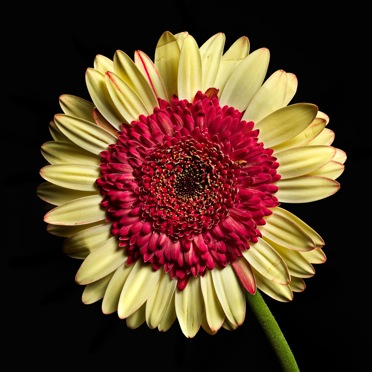
\includegraphics[scale=0.22]{img/originalFlower}}
     \subfigure[Edges]{\label{lssample}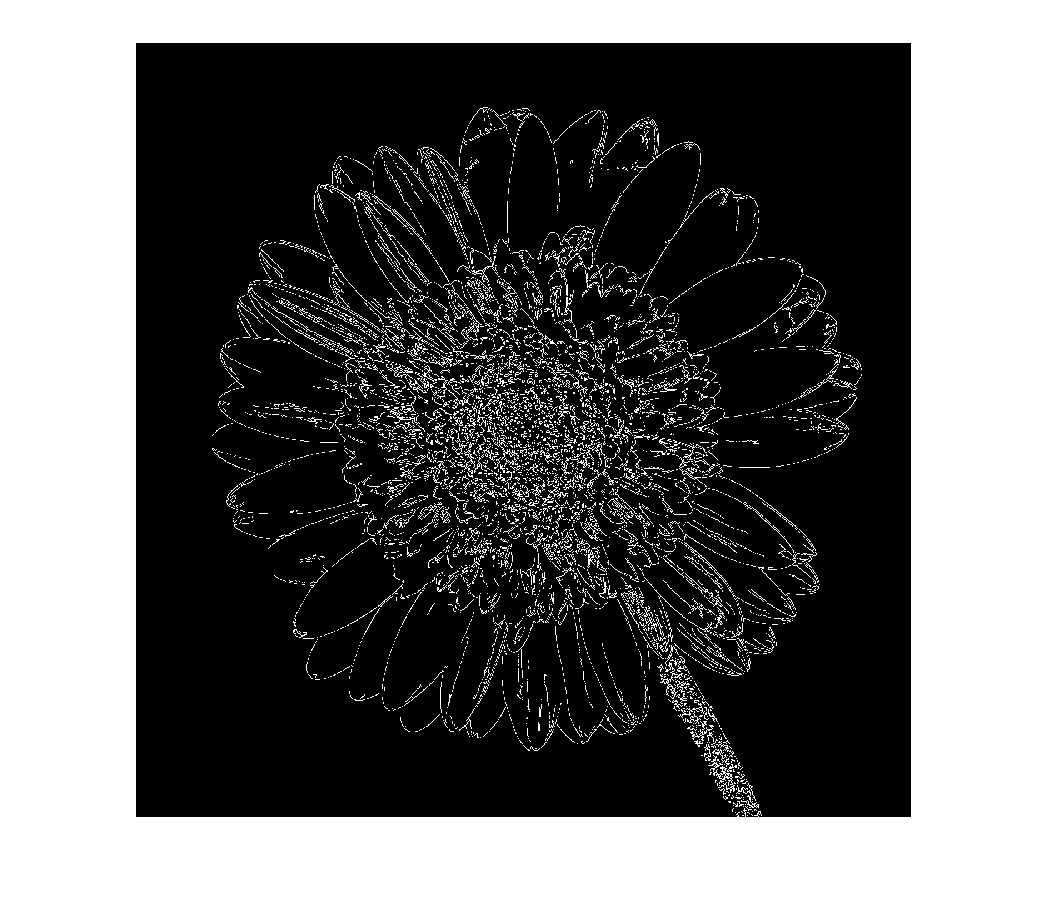
\includegraphics[scale=0.22]{img/edgesFlower}} 
     \subfigure[Corners]{\label{lssample}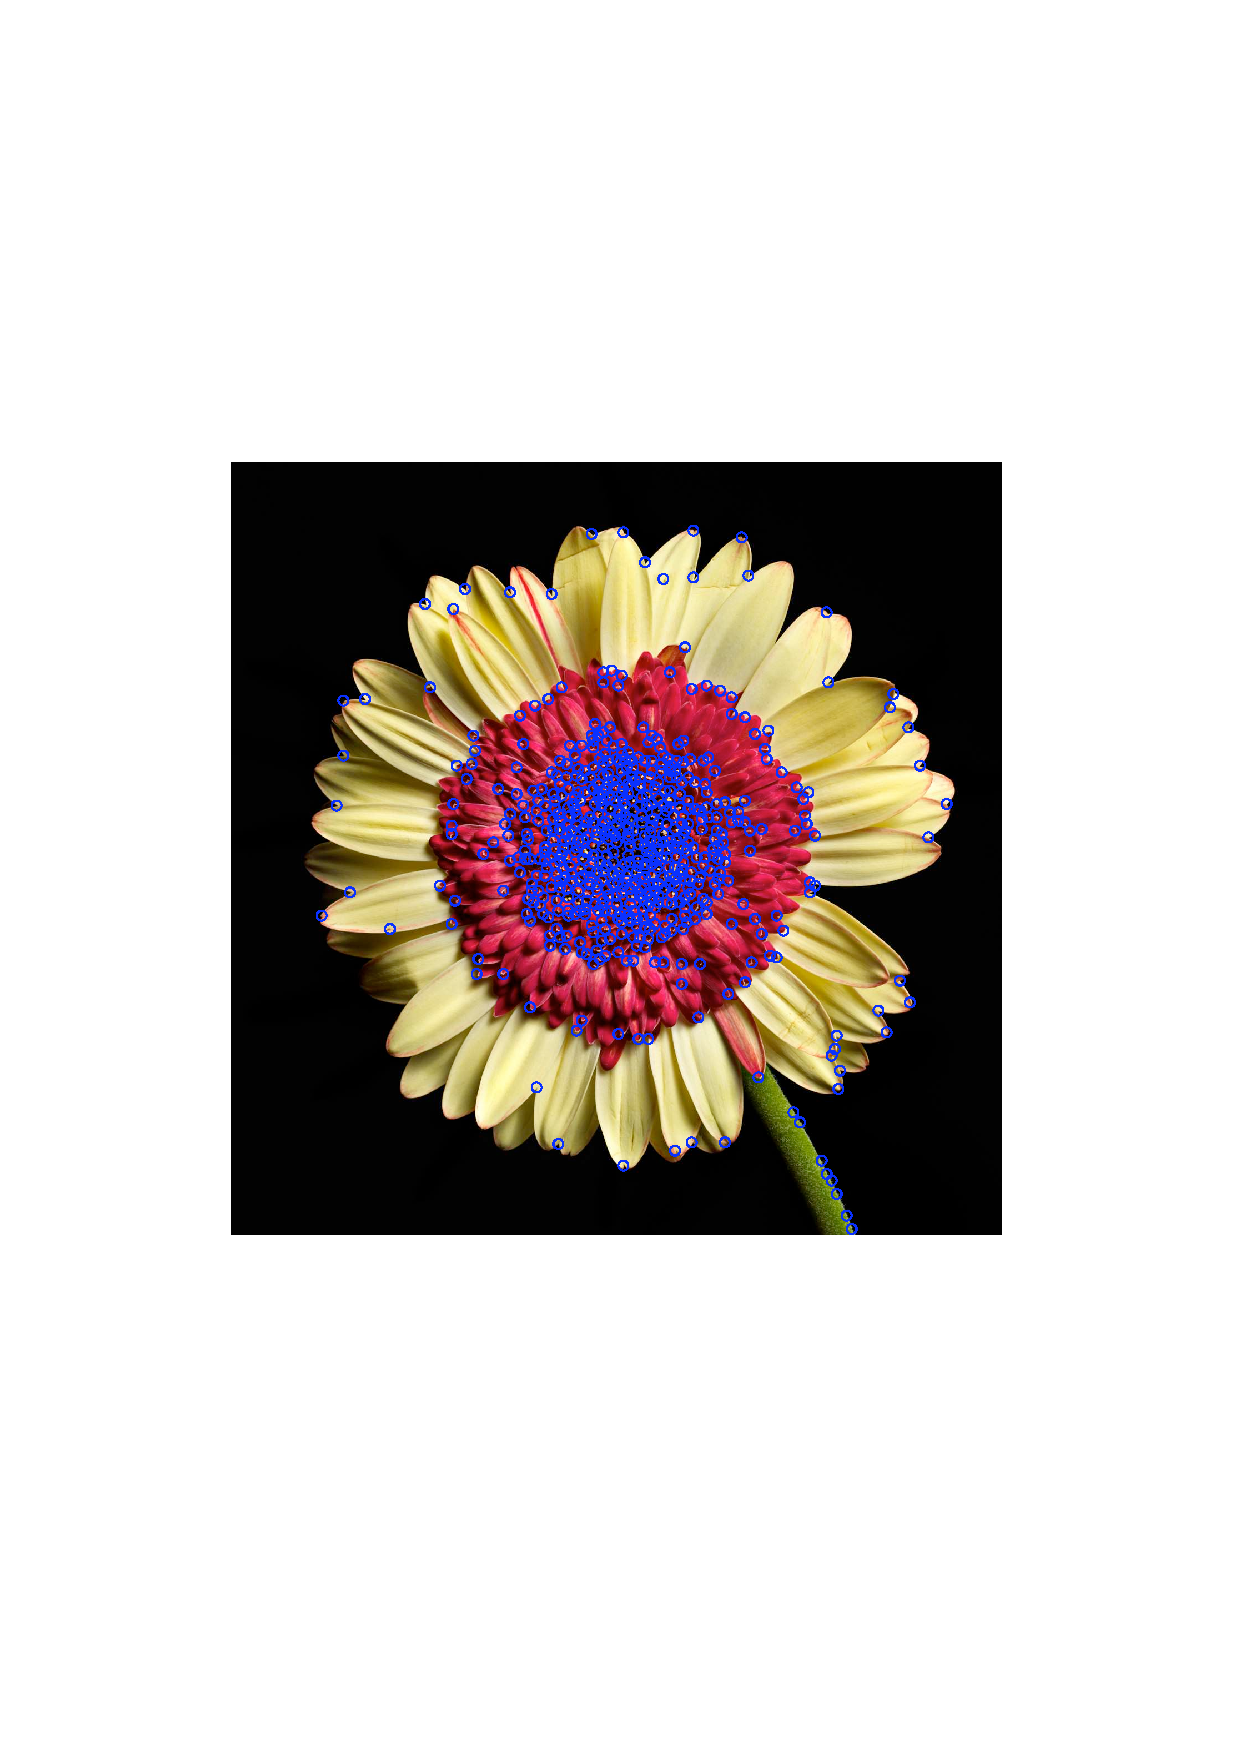
\includegraphics[scale=0.22]{img/cornersFlower}}  
     \subfigure[Hue]{\label{lssample}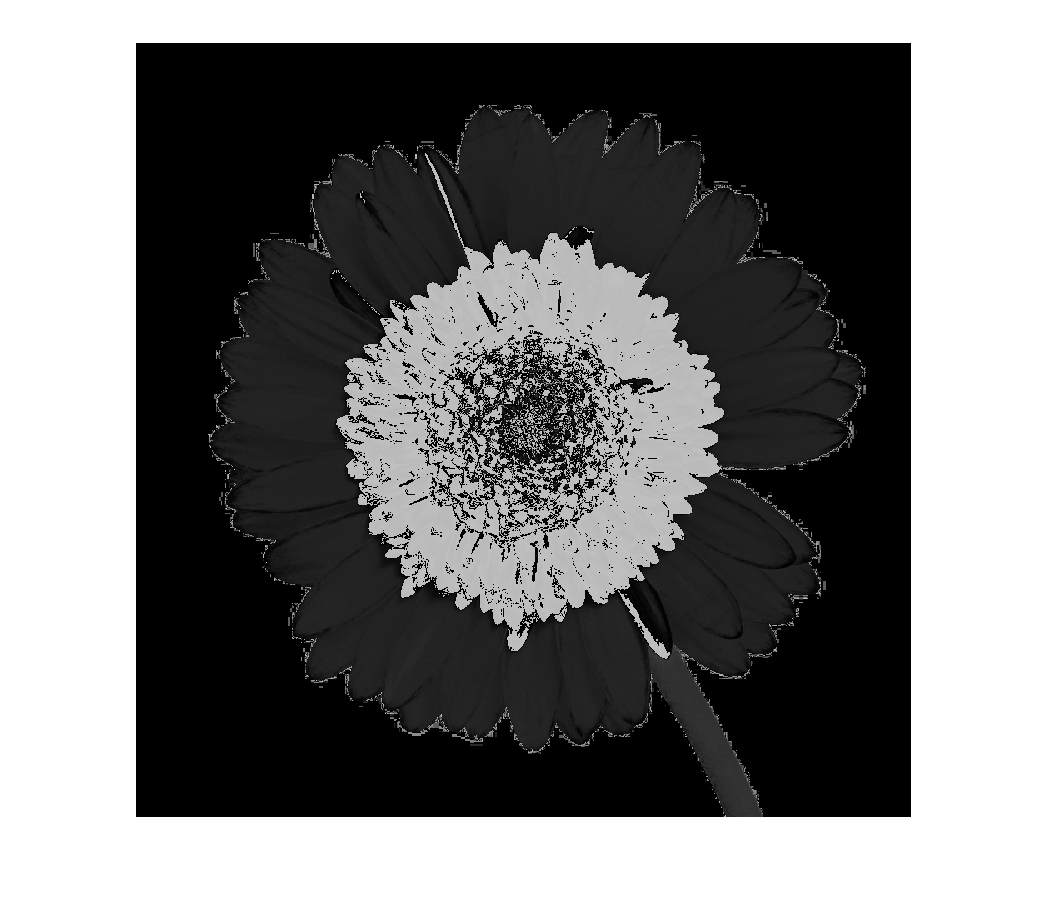
\includegraphics[scale=0.22]{img/hueFlower}}           
     \subfigure[Saturation]{\label{lssample}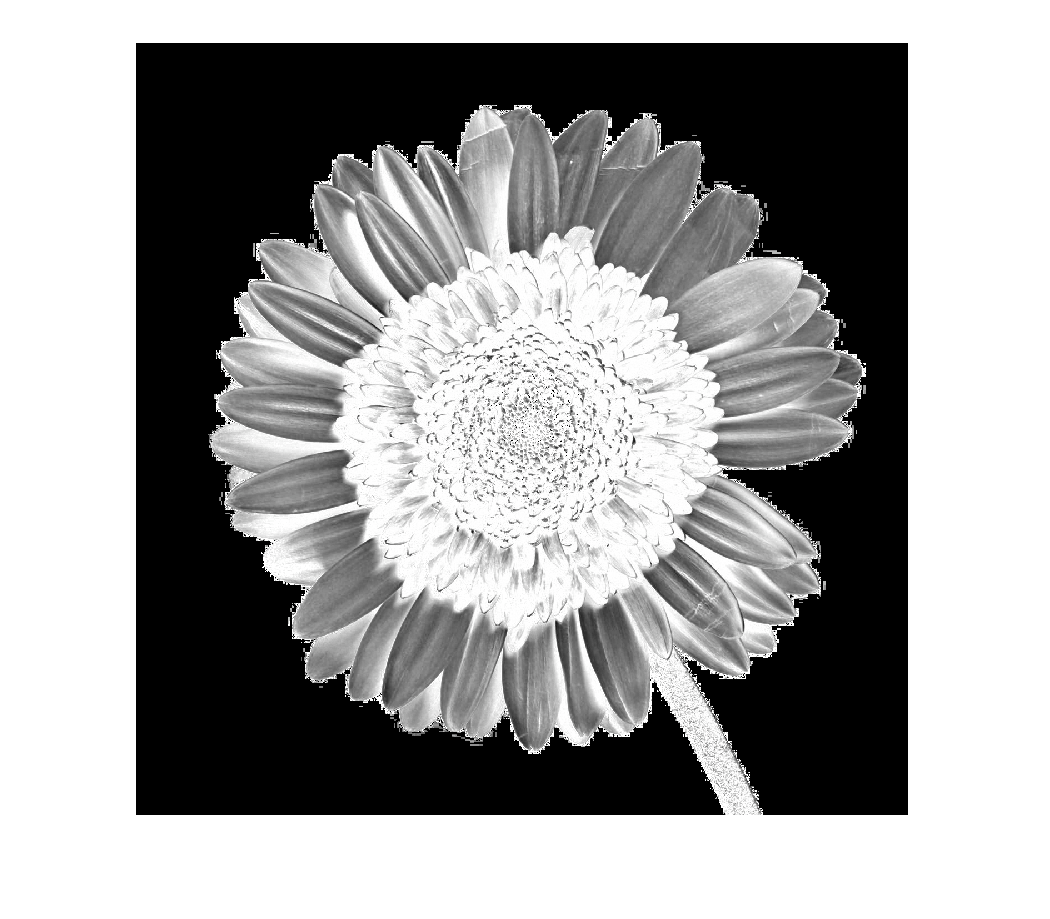
\includegraphics[scale=0.22]{img/satFlower}}           
     \subfigure[Value]{\label{lssample}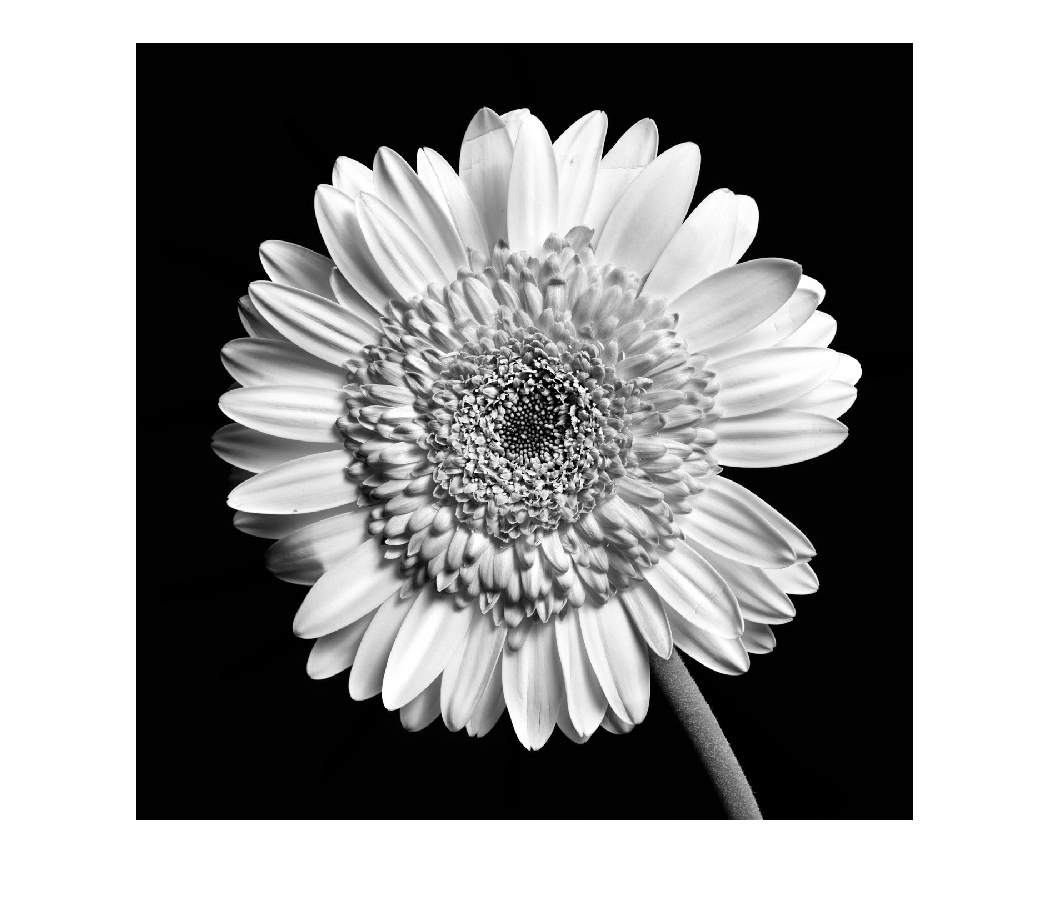
\includegraphics[scale=0.22]{img/valueFlower}}
     \subfigure[Intensity]{\label{lssample}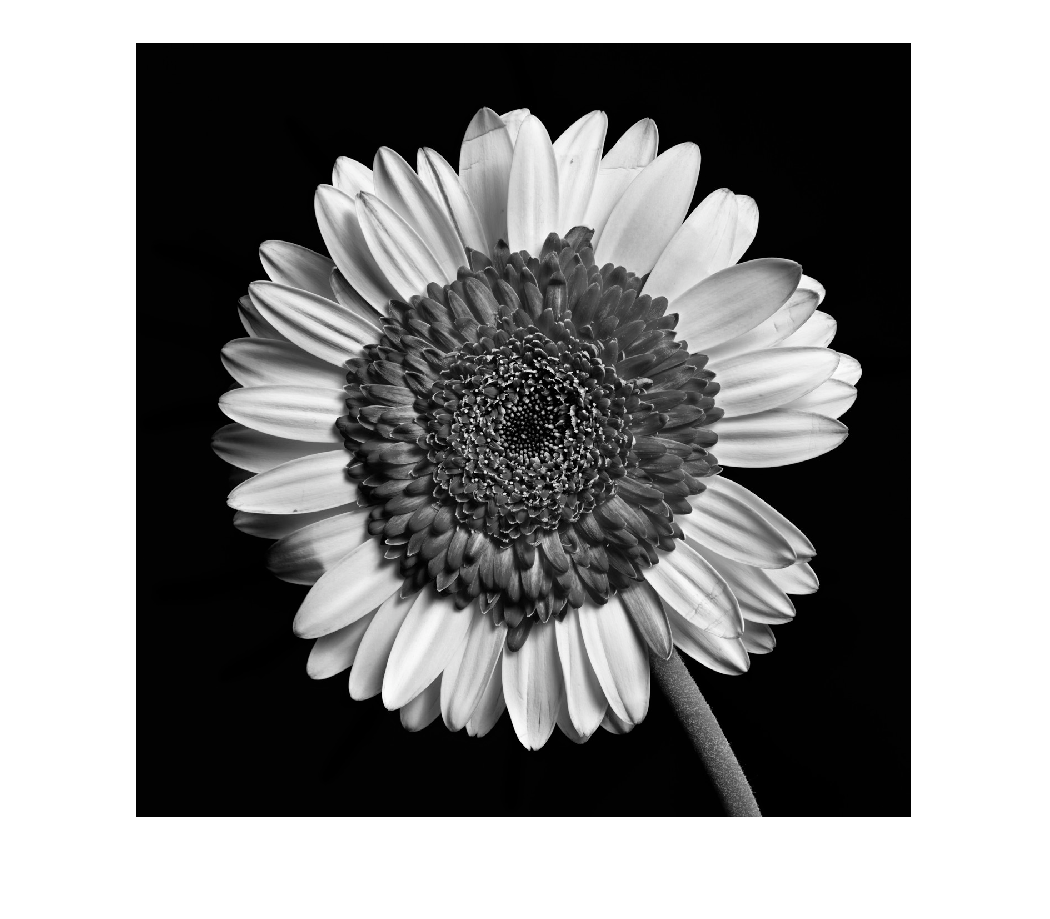
\includegraphics[scale=0.22]{img/intFlower}}                               
     \subfigure[Red]{\label{lssample}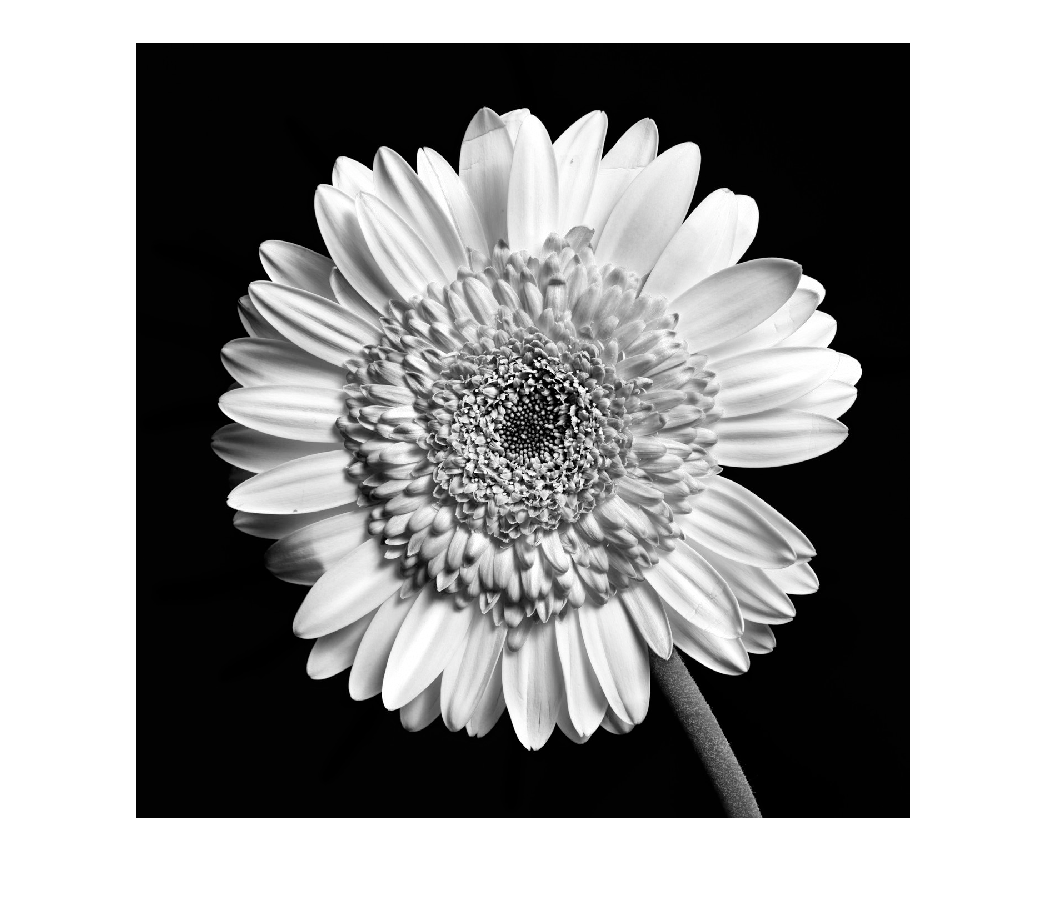
\includegraphics[scale=0.22]{img/redFlower}}
     \subfigure[Green]{\label{lssample}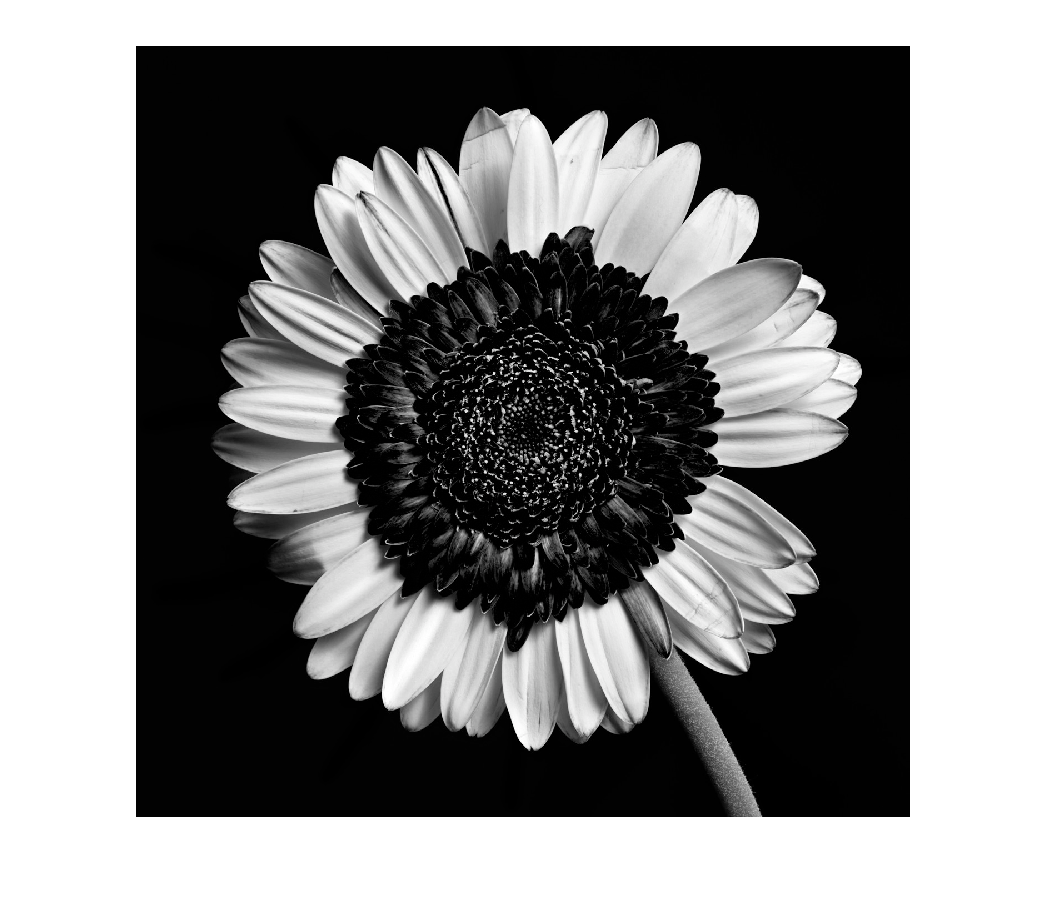
\includegraphics[scale=0.22]{img/greenFlower}}
     \subfigure[Blue]{\label{lssample}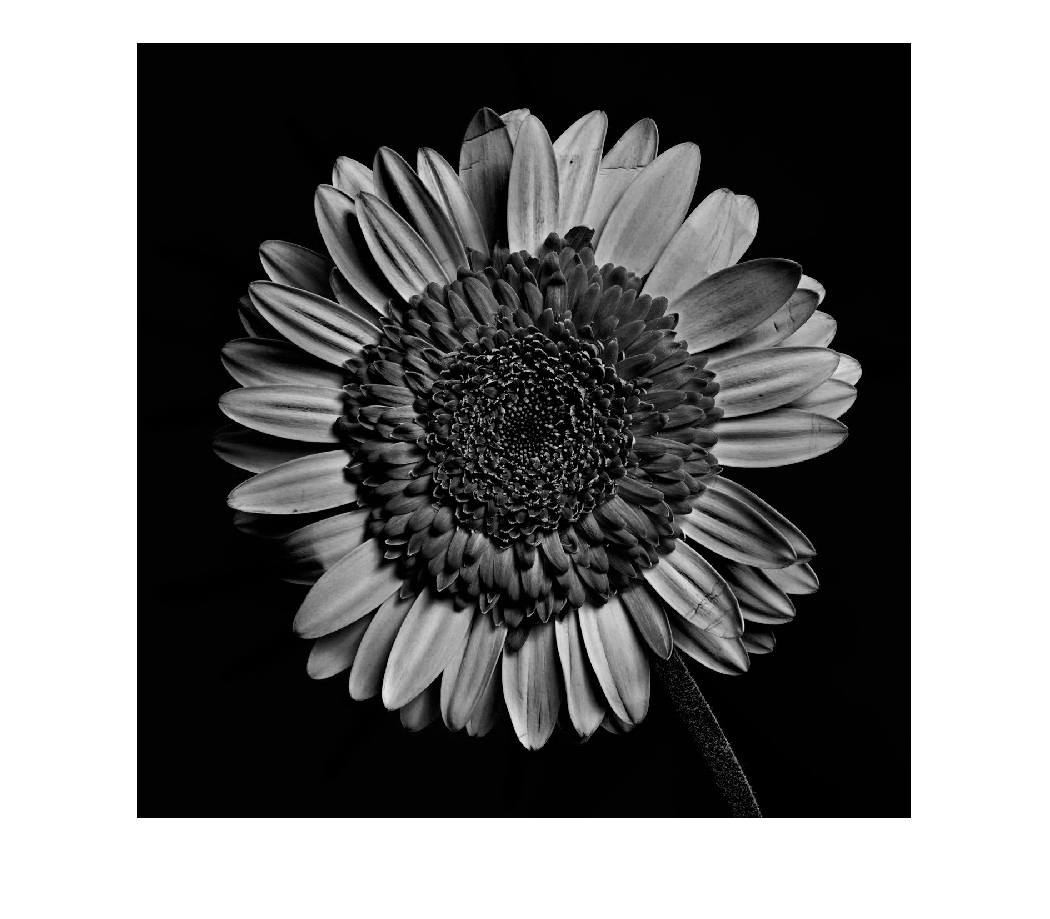
\includegraphics[scale=0.22]{img/blueFlower}}

  \end{center}
  \caption{Illustration of different statistical features}
  \label{featureImg}
\end{figure}


The features described above only contain global information about images. In order to capture localized information as well, several of the features described above are also extracted from different regions of the image. The regions of the image are obtained by dividing the image along both dimensions into NxM equal-sized regions. Since feature values will most likely vary from region region, these compositional features should provide valuable additional information about an image. Figure \ref{gridImage} shows an example of 

\begin{figure}
\label{gridImage}
\begin{center}
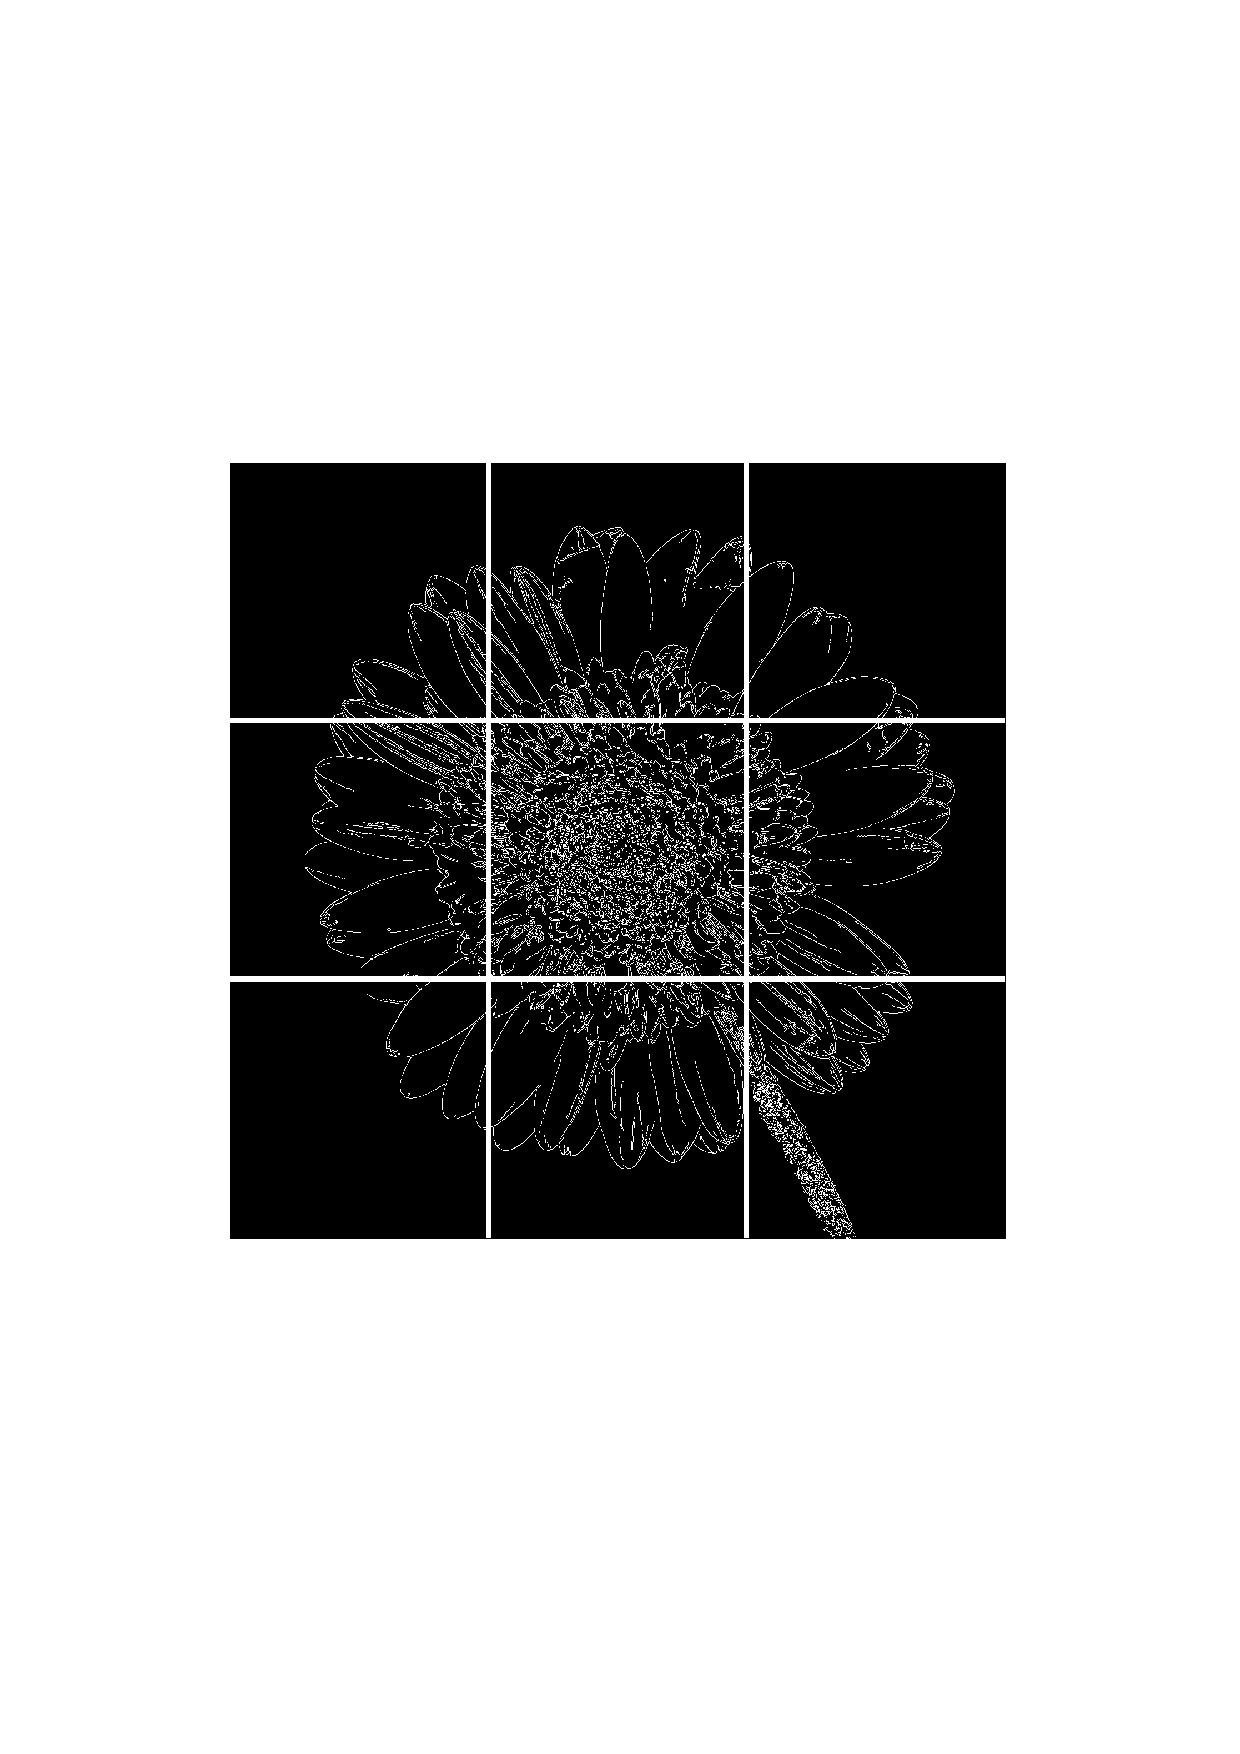
\includegraphics[scale=0.4]{img/gridEdgesFlower}   
\end{center}
\end{figure}
%\textbf{add reference to opencv somewhere}


%\subsubsection{Weibull, this subsubsubsection can be made normal text, but we can do that later}
%The contrast of natural image statistics has been shown to conform to Weibull-shaped probability distributions \cite{Weibull_physical}. Furthermore, when images do not adhere to this distribution, the images in question are mashups of multiple sub-images which themselves do conform to the Weibull distribution. In addition to this property of natural images, it has been proposed that the parameters for the Weibull distribution form a basis for the description of texture in images \cite{Weibull_6}. There is indeed evidence that the human visual system is capable of approximating the parameters of the Weibull distribution \cite{Weibull_brain}. Last the two most important parameters of the Weibull distribution, when it comes to natural images have a straight forward interpretation, the shape parameter the describes the resemblance to other probability distribution, from a power-law to the normal distribution, where the scale describes the how wide the distribution is. Therefore we included the maximum likelihood estimation of the Weibull-distribution for contrast of the image as used for \cite{Weibull_6} in our Feature extraction toolbox, unfortunately this seemed to give unstable results, therefore we later eliminated it. 

\paragraph{\textit{Cognitively-inspired features} \label{proposed-cognitive}}
One of the more recent trends in computer vision research in the pursuit of human-like capability is the coupling of cognition and vision into cognitive computer vision. The term cognitive computer vision has been introduced with the aim of achieving more robust, resilient, and adaptable computer vision systems by endowing them with a cognitive faculty: the ability to learn, adapt, weigh alternative solutions, and develop new strategies for analysis and interpretation.

Recent studies focused on computational models of focal visual attention. Attention has been seen to influences the processing of visual information even in the earliest areas of primate visual cortex. Even more, it has been discovered that the interaction of bottom-up sensory information and top-down attentional influences creates an integrated \textit{saliency map}, that can be defined as a topographic representation of relative stimulus strength and behavioral relevance across visual space \cite{Saliency_WWHW}. This map enables the visual system to integrate large amounts of information, even from outside the fovea, because it provides an efficient coding scheme for the potentially most relevant information in the sensory input. 
An important model based on this theory is the one provided by Itti, Koch and Niebur \cite{Itti_review}\cite{Itti_model}. The model tries to mimic the properties of primate early vision. Despite its simple architecture the model is capable of strong performance with complex natural scene.
The model work as follow: an input image is decomposed through several pre-attentive feature detection mechanisms which operate in parallel channels over the entire visual scene, and four conspicuity maps (color, orientation, intensity and skin) are created. After few different intermediate steps, the model finally combines the four conspicuity maps into a unique saliency map. 

Til now the saliency map has been used as information channel in scene understanding and object recognition. In this reasearch, image features have extracted from the map and then used in the classification and visualization task. Features that have been extracted from those maps are: \textit{Shannon entropy} of the five maps, \textit{Standard deviation} of the distribution of attention in the saliency map, \textit{Location} of the most salient points (defined as the centers of the most salient regions) and \textit{Skin intensity} of the skin map. Skin is not a default channel in the Itti's model, but it has been found out to be really interesting and useful in devianART to distinguish artists and artworks, where there is a huge presence of photographer that create nude art. 


\begin{figure}[h!]
\centering
\subfigure[]{
\includegraphics[scale=0.135]{Saliency_images/A_landscape_pic_with_a_loli_bg_by_CroireIgeen.png}\label{fig:saliencyimg1}}
\subfigure[]{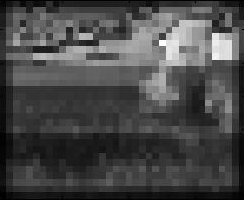
\includegraphics[scale=0.33]{Saliency_images/color.PNG}\label{fig:saliencyimgc1}}
\subfigure[]{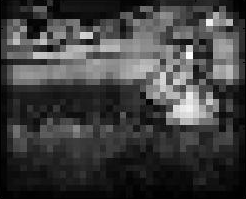
\includegraphics[scale=0.33]{Saliency_images/intensity.PNG}\label{fig:saliencyimgc2}}
\subfigure[]{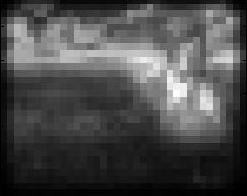
\includegraphics[scale=0.33]{Saliency_images/orientation.PNG}\label{fig:saliencyimgc3}}
\subfigure[]{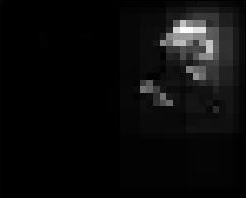
\includegraphics[scale=0.33]{Saliency_images/skin.PNG}\label{fig:saliencyimgc4}}
\subfigure[]{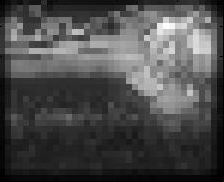
\includegraphics[scale=0.36]{Saliency_images/sm.PNG}\label{fig:ex_saliencymap}}

\caption{Example of saliency maps. (f) shows the final saliency map, while (b), (c), (d) and (e) show the conspicuity maps for color, intensity, orientation and skin respectively.}
\end{figure}


\subsubsection{Classification}

%REVIEW THIS PART!!!
%- FOCUS ON DESCRIBING WHY WE NEED TO CLASSIFY IN OUR PROJECT
%- WHICH CLASSIFIER WE USE AND FOR WHAT REASONS (WE CAN REFER TO SOME PAPERS ////////////////////////// THAT SHOW RESULTS IN VISUAL CLASSIFICATION)
%- EXPLAIN THE EVALUATION MEASURE USED (introduce precision and recall, but they are intermediate measure used to compute the F-Measure!!! P&R never appear in the final results)
%- INTRODUCE THE IDEA OF A DATASET WITHOUT GROUND TRUTH AND WITH THE NEED OF USING 5-FOLD CROSS VALIDATION (check the paper I sent you! ;) )
%- SAY SOMETHING ABOUT FEATURE SELECTION AND HOW WE DO IT! (refer to the description above!! remember feature extraction and classification are in the SAME section and they work together)
%- HOPE THOSE INFORMATION CAN BE USEFUL! ;)

The most important aspect in this project is to describe images, artists or categories using the features that were extracted.
In this approach, classifiers are used to give a performance score to a set of features that is used to either describe an artist or a category.

\paragraph{Data normalization}

Classifiers improve their classification performance when the dataset that is used is normalized.
In this case every extracted feature in the dataset has a different value range, it is important to translate all the different ranges to one defined value range so that the data is normalized.

\begin{equation}
\label{minmax}
y_n=\frac{x_n - \max(x_n)}{\max(x_n)-\min(x_n)} * (B-A)
\end{equation}

Equation \ref{minmax} shows the Min/Max normalization that was used to normalize the data in our approach.
In this equation $A$ and $B$ represents the range [$A$,$B$] where the values are normalized to.
$x$ represents the unnormalized values of feature $n$ whereas $y$ represents the normalized values of feature $n$.

\paragraph{Classifiers}
In our approach, four different classifiers were incorporated to calculate the performance of a set of features.
All classifiers were chosen based on their performance in earlier work except for the Nearest Mean classifier.

The \textit{k-Nearest Neighbour} \ref{korn1996fast} classifies an artwork based on the training examples that are close to it.
The euclidian distance is used here to measure how far a training example is located from the artwork.

The \textit{Naive Bayes} \ref{keren2003recognizing} first divides the value range for each feature in $n$ bins.
It then counts the frequency of a training example for each of the classes in every bin and uses that to classify an artwork belonging to the class that gives the maximum posterior probability.

The \textit{Nearest Mean} classifies an artwork based on the euclidian distance to the mean of a class.
The classifier was chosen because it might give a high performance for when the right features are used to describe a class.
This is because the right features of a class will make the artwork of that class cluster.

At last the \textit{Support Vector Machine} \ref{chapelle1999svms} classifies an artwork using a model created with training examples.
The model represents the training examples in a way that separates the two classes by a clear gap that is as wide as possible.
The artwork is classified by the model based on which side of the gap they fall on.

\paragraph{Feature Selection}
The classifiers are used in our approach to compute the performance score of a set of features.
On the other hand a feature selection algorithm is used to extract a set of features out of all the features that were pre-computed.
This is important because we want to have the smallest set of features to describe a class.

The feature selection in our approach starts by selecting the most informative feature and for each step iteratively adds the next most informative feature to it in a greedy fashion.

\begin{equation}
\label{featureselect}
F := F \cup f, where f: \max{J(f_i)} \wedge f_i \epsilon F
\end{equation}

Formula \ref{featureselect} is a formally written representation of this algorithm.
In this formula, $F$ represents the entire feature set, $f$ one single feature and $J$ the criterion that is used to define if a feature is informative.

The inter-intra distance is used as the criterion to define if a feature is informative.
This criterion works by measuring the inner-scatter of a class over a feature and measures it against the scatter of that class around the average of the feature.
For a two class problem like in our approach the inter-intra distance can be written as:

\begin{equation}
\label{interintra}
J = \frac{|m_1-m_2|}{\sqrt(s^2_1 + s^2_2)}
\end{equation}

In this equation $m_1$ and $m_2$ are the average mean of class 1 and class 2, $s_1$ and $s_2$ are the standard deviations of those classes.
This equation is also equivalent to the Fisher criterion \ref{malina1981extended}.

\paragraph{Performance measures}
A performance measure is needed to assign a performance score to a set of features.
Because our approach requires the need of classifiers, it is arbitrary that the performance measure is the same as the evaluation measure of the classifier.

Every prediction of the classifier is labeled into one of the following four types,
depending on whether or not the classification was correct:

\begin{tabular}{r|c|c|}
\multicolumn{1}{r}{}
 &  \multicolumn{1}{c}{predicted positive}
 & \multicolumn{1}{c}{predicted negative} \\
\cline{2-3}
positive & \textbf{tp} (true positive) & \textbf{fp} (false positive) \\
\cline{2-3}
negative & \textbf{fn} (false negative) & \textbf{tn} (true negative) \\
\cline{2-3}
\end{tabular}

With these standard classification measures two more evaluation measures can be computed from it.
These are the precision and the recall.
The $precision$ is defined as the number of relevant artwork correctly classified as positive divided by the total number of positive classified artwork.

\begin{equation}
Precision = \frac{tp}{tp + fp}
\end{equation}

The $recall$ is defined as the number of relevant artwork correctly classified as positive divided by the total number of positive examples in the dataset.

\begin{equation}
Recall = \frac{tp}{tp + fn}
\end{equation}

The precision and recall are measures that are used to compute the $F-measure$.
This measure is the weighted harmonic mean of the precision and recall and can be defined as:

\begin{equation}
F_\beta = \frac{(1+\beta)^2 (Precision * Recall)}{(\beta ^2 * Precision) + Recall}
\end{equation}

In our case we use $\beta$=1 which means that the precision and recall are evenly weighted.

	\subsection{Visualization}
	\subsubsection{Previous work}
Image features and information visualization are both research fields that have received great interest.
Research that combines both fields is largely coming from the image retrieval field, focussing on efficient methods to retrieve images from (large) image collections.

Musha et al~\cite{musha1998interface} developed a visualization method and an interface for image retrieval.
In their method, principal component analysis (PCA) is dynamically applied to the to image features of the retrieved images in order to determine their eigenspace and the retrieved images are displayed in that space.
Statistical experiments showed that heir method effectively decentralizes the retrieved images over the two-dimensional space.

Chen et al.~\cite{chen2000content} compared and analyzed a number of Pathfinder networks of images generated based on low-Ievel image features (color, texture and shape).
Salient structures of images are visualized according to features extracted from color, texture, and shape orientation.

Schneidewind et al~\cite{schneidewind2004approach} presented a visualization technique that aims to provide a tool to analyze a mismatch between the user�s perception and the system�s calculation of similarity.
They combine techniques of visual image retrieval and information visualization to acquire insight into the extracted feature data.
They implemented three visualization techniques to present feature data on three different levels of abstraction: Data Table, a Parallel Coordinate Plot, and a Color Space Plot.

%Imo et al~\cite{imo2008interactive} propose to make content based image retrieval systems more �transparent� by visualization of the employed features.
%Since non-experts should be able to operate the CBIR system, they argue that features should be visualized as prototypical, artificial images, rather than feature-specific visualizations.
% sidetrack?

Yang el al~\cite{yang2006semantic} propose a scalable semantic image browser by applying existing information visualization techniques to semantic image analysis.
The system consists of multiple visualization components that allows effective high dimensional visualization without dimension reduction.
The Multi-Dimensional Scaling image view maps image miniatures onto the screen based on their content similarities using a fast MDS algorithm.
Interactions are provided to reduce clutter.% (reordering, dynamic scaling, relocation, distortion, showing original image, zooming and panning).
The Value and Relation content view visually represents the contents of the whole image collection.
The correlations among different contents within the image collection, as well as detailed annotations of each image, are visually revealed in this view.
The concept-sensitive image content analysis technique was used as automatic annotation engine.
This technique abstracts image contents by automatically detecting the underlying salient objects in images and associating them with the corresponding semantic objects and concepts according to their perceptual properties.


\section{Toolkit}
\begin{figure}[htb]
  \centering
  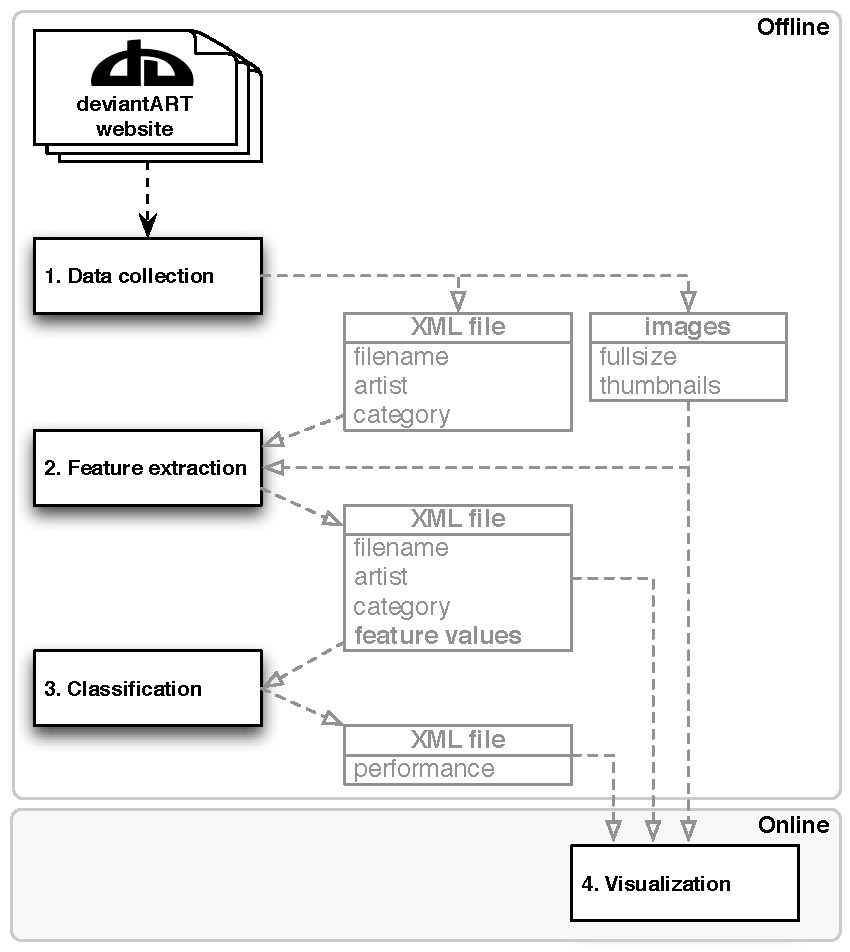
\includegraphics[width=1\linewidth]{img/components.pdf}
  \caption{Interaction between the four components of the toolkit.}
  \label{fig:components}
\end{figure}

Our toolkit consists out of four components and each component is replacable.
Each component writes the output (e.g. image information and features) to a XML file.
The first three components are all executed \textit{offline} (precalculated), while the visualization component allows \textit{online} interaction with the images, features and classification results.
For a complete overview see Fig.~\ref{fig:components}.

% toolboxes used
\subsection{Data collection}
It deals with downloading information and galleries from the deviantART website and it can easily be replaced to allow the toolkit to be flexible and be able to deal with different art community webpages

DeviantArt does not provide a web API to download images and therefor the backend links of the galleries to the RSS XML files were followed to access
the image data. For each image general information such as category, deviantART link and filename are stored, and the full image and 
thumbnails are downloaded.

For the network information collection the friends pages 
of the users are parsed. No RSS XML files are provided by deviantART for this
information, instead the HTML pages were parsed.


%When working with images, it is usually not possible to work with the raw image data (the pixel values). The reason for this is the high dimensionality of images, which can easily exist in a space of more than a million dimensions. By extracting features from images, they can be represented in a lower dimensional feature-space.  This feature extraction process has several advantages:
%\begin{itemize}
%\item The data becomes computationally easier to work with due to the smaller number of dimensions
%\item By using the right features, the data becomes more suitable for generalization across images
%\item Reducing the dimensionality makes it easier to visualize sets of images
%\item Features can have an intuitive basis, which makes it easier for non-computer-scientists to analyze (sets of) images
%\end{itemize}

%% Computer vision is an important and maturing engineering science. It underpins an increasing variety of applications that require the acquisition, analysis, and interpretation of visual information.
%In the extraction of image features, a distinction was made between low-level statistical features and higher level cognitive-based features....

%\subsubsection{Statistical features}
%As statistical features, many relatively simple low-level features were extracted from the images.
%The first type of statistical features that were used are color-based features, which should capture the color-usage in the artwork. Many artists produce collections of art pieces with similar colors, and should therefore be (partially) distinguishable with color-based features. For each of the three RGB channels, an average and median is calculated over all the channel values. Let $\{\mathbf{x}_{m,i,c} \}_{i=1\dots n}$ be the pixel values for image $m$ in color channel $c \in \{R,G,B \}$. The average in channel $c$ of image $m$ is then given by 

%\begin{equation}
%\label{avgChannel}
%\mu_c(\mathbf{x}_{m}) = \frac{1}{n}\sum_{i=1}^{n} \mathbf{x}_{m,i,c} 
%\end{equation}
%The median in channel $c$ is given by 
%\begin{equation}
%\label{medChannel}
%\tilde{\mathbf{x}}_{m,c} = \mathbf{x'}_{m,k,c}
%\end{equation}
%where $\{\mathbf{x'}_{m,i,c}\}_{i = 1\dots n}$ are the sorted pixel values of channel $c$ and $k = \mbox{round}(n/2)$.
%The image is also converted into the HSV color space, from which the average and median is extracted for each channel as defined in equations \ref{avgChannel} and \ref{medChannel}. The Hue channel is given by: 

%$H_{m,i} = \left\{ 
%\begin{array}{ll}
%0 & \mbox{if $C_{m,i} = 0$};\\
%60 \left(\frac{G_{m,i}-B_{m,i}}{C_{m,i}} \mbox{mod} 6 \right) & \mbox{if $M_{m,i} = R_{m,i}$};\\
%60 \left(\frac{B_{m,i}-R_{m,i}}{C_{m,i}} + 2 \right) & \mbox{if $M_{m,i} = G_{m,i}$};\\
%60 \left(\frac{R_{m,i}-G_{m,i}}{C_{m,i}} + 4 \right) & \mbox{if $M_{m,i} = B_{m,i}$}; \\
%\end{array} 
%\right\}$
%Where $M_{m,i} = \max(R_{m,i},G_{m,i},B_{m,i})$ and $C_{m,i} =  M - \min(R_{m,i},G_{m,i},B_{m,i})$. The value channel is given by $V_{m,i} =  M_{m,i}$ and the saturation channel is  by $S_{m,i} = \frac{C_{m,i}}{V_{m,i}}$

%The second group of features is the edge to pixel and corner to pixel ratio. Let $\{\mathbf{x}_{m,i} \}_{i=1\dots n}$ be the pixel values of the binary edge-image produced by applying a Canny edge detector[REF] on image $m$. The edge to pixel ratio of image $m$ is then computed as $f_{e,m} = \frac{1}{n}\sum_{i=1}^{n} \mathbf{x}_{m,i} $. Let $\{\mathbf{y}_{m,i} \}_{i=1\dots n}$ be the pixel values in the binary corner image produced by a corner detector that are either $1$ if the pixel is a corner or $0$ otherwise. The corner to pixel ratio of image $m$ is then computed as  $f_{c,m} = \frac{1}{n}\sum_{i=1}^{n} \mathbf{y_{m,i}} $. These two features should be helpful in distinguishing many photography artworks from other genres such as cartoons and manga. The latter two tend to have large patches of plain color patches, which will decrease the amount of edges and corners. They are also somewhat indicative to the type of scenes in photography. A blue sky will not produce many edges or corners, whereas a busy street will.  

%%$v : R^2 \rightarrow \{0,1\}$
%%calculated by performing Canny edge detection on the image to construct an image of edges. The number of edge pixels in this image, divided by the total number of pixels is then used as a feature. The same is done using a corner detector. 

%For the final group of features, the artworks are converted from RGB image $m$ to a greyscale intensity image $I_m$ by taking for each pixel $i$, a weighted sum of the R,G and B channels: $I_{m,i} = 0.2989R_{m,i} + 0.5870G_{m,i} + 0.1140B_{m,i} $. Let $\{\mathbf{z}_{m,i}\}_{i=1\dots n}$ be the pixel values of the greyscale intensity image of image $m$. The average intensity feature is then calculated as $f_{\mu_{I_m}} = \frac{1}{n} \sum_{i = 1}^{n} \mathbf{z}_{m,i}$ and the median intensity as $\tilde{I}_m = \mathbf{z'}_{m,k}$, where $\{\mathbf{z'}_{m,i}\}_{i = 1\dots n}$ are the sorted pixel values and $k = \mbox{round}(n/2)$. These values give information about the lightness or darkness of artworks. The intensity variance feature is computed as $\mbox{Var}(I_m) = \frac{1}{n} \sum_{i=1}^n \mathbf{z}_{m,i}$, which reacts to the contrast between lightness and darkness in images. Finally the entropy of the intensity is calculated as follows. $H(I_m) = -\sum_{u = 1}^{j} \hat{p}_u \log_2(\hat{p}_u) $, where $\{\hat{p}_u(\mathbf{z}_m)\}_{u = 1 \dots j}$ are the histogram bins of the intensity values and are defined as $\hat{p}_u(\mathbf{z}_m) = \sum_{i=1}^n \delta[b(\mathbf{z}_{m,i}) - u] $. The function $b : R \rightarrow \{1 \dots j \}$ returns the index of the bin of the input pixel value in the intensity space and $\delta[g] = 1$ if $g = 0$, otherwise $0$. This feature somewhat characterizes the texture in an image.  

%The features described above only contain global information about images. In order to capture localized information as well, several of the features described above are also extracted from different regions of the image. The regions of the image are obtained by dividing the image along both dimensions into NxM equal-sized regions. Since feature values will most likely vary from region region, these compositional features should provide valuable additional information about an image. 

%\textbf{add reference to opencv somewhere}


%\begin{itemize}
%\item Edge ratio: description
%\item Corner ratio: description
%\item etc...
%\end{itemize}
%\subsubsection{Weibull, this subsubsubsection can be made normal text, but we can do that later}
%The contrast of natural image statistics has been shown to conform to Weibull-shaped probability distributions \cite{Weibull_physical}. Furthermore, when images do not adhere to this distribution, the images in question are mashups of multiple sub-images which themselves do conform to the Weibull distribution. In addition to this property of natural images, it has been proposed that the parameters for the Weibull distribution form a basis for the description of texture in images \cite{Weibull_6}. There is indeed evidence that the human visual system is capable of approximating the parameters of the Weibull distribution \cite{Weibull_brain}. Last the two most important parameters of the Weibull distribution, when it comes to natural images have a straight forward interpretation, the shape parameter the describes the resemblance to other probability distribution, from a power-law to the normal distribution, where the scale describes the how wide the distribution is. Therefore we included the maximum likelihood estimation of the Weibull-distribution for contrast of the image as used for \cite{Weibull_6} in our Feature extraction toolbox, unfortunately this seemed to give unstable results, therefore we later eliminated it. 

%\subsubsection{Cognitively-inspired features}
%As it has already been explained in the previous work, a saliency map enables the visual system to integrate large amounts of information. Til now those information has been used in scene understanding and object recognition. In this reasearch, image features have extracted from the map and then used in the classification and visualization task.  
%It has been used the Itti's model \cite{Itti_model} due to its low computentional time and the existense of a free toolkit \footnote{http://www.saliencytoolbox.net/} made by Dirk Walther.
%The model work as follow: an input image is decomposed through several pre-attentive feature detection mechanisms which operate in parallel channels over the entire visual scene, and four conspicuity maps (color, orientation, intensity and skin) are created. After few different intermediate steps, the model finally combines the four conspicuity maps into a unique saliency map. 
%The toolkit has been used to create the saliency maps and the intermediate maps (color, intensity, orientation and skin). Features that have been extracted from those maps are: \textit{Shannon entropy} of the five maps, \textit{Standard deviation} of the distribution of attention in the saliency map, \textit{Location} of the most salient points (defined as the centers of the most salient regions) and \textit{Skin intensity} of the skin map. Skin is not a default channel in the Itti's model, but it has been found out to be really interesting and useful in devianART to distinguish artists and artworks, where there is a huge presence of photographer that create nude art. 

\subsection{Feature extraction}
The feature extraction is implemented in the MATLAB programming language. Part of the statistical feature calculations were done using MATLAB-compiled openCV [REF] code to speed up the feature extraction. openCV was used for color-space transformations, edge,corner and face-detection.

As it has already been explained in section \ref{proposed-cognitive}, the research focused also on the extraction of some cognitive-inspired features. First a saliency map and 4 conspicuity maps (color, intensity, orientation and skin) are computed and then the features are extracted. To create the maps it has been used the Itti's model \cite{Itti_model} due to its low computentional time and the existense of a free toolkit \footnote{http://www.saliencytoolbox.net/} made by Dirk Walther. Both the toolkit and the code to extract the features are written in Matlab. 

The XML-processing was done using an open-source XML-toolkit for MATLAB~\footnote{\url{http://www.mathworks.com/matlabcentral/fileexchange/4278}}~\cite{geusebroek2005six}.



\subsection{Classification}
An important aspect of analyzing images is to determine what makes them distinct.
In this tookit, classification is used to compare image sets and extract the image features that best separates them.
This knowledge can be used to describe the art style of an artist or even determine if there is an artist that uses an unique style.
Also classification can be extended to other category level to determine what the image features of a category are.

\subsubsection{Pre-processing}
Before classifiers can be used to find image features, several pre-processing steps are required on the dataset.

Naturally, functions that read in XML files containing the feature values, convert it to a dataset and splitting it into a train and test set are incorporated.
Also Min/Max normalization can be used on the dataset.
Normalization is important because the features that were extracted all uses different ranges of values, by scaling these values to the same range(e.g. [-0.5,0.5]), classifiers are more effective in their task to find image features that separates a class from the other classes.

Furthermore filtering on classes and features can be performed on the dataset, this is to provide flexibility in a way that the user can do classification on just a few interesting classes or features instead of everything that is inside the dataset.

\subsubsection{Classifiers}
The classification part of the toolkit is implemented using the Matlab environment. In total there are four different classifiers that be called upon.

\begin{itemize}
	\item \textbf{k-Nearest Neighbour}: It classifies images based on the closest training examples.
	This classifier uses a parameter $k$ that can be optimized. 
	The parameter indicates how many of the training examples the classifier should compare the new image with before it can classify to what class an image belongs to.
	\item \textbf{Naive Bayes}: It calculates the probability of a new image belonging to a class.
	This classifier takes every feature seperately and divide it into $N$ bins, it will then count the number of training examples for every class in all the bins and uses this to compute the posterior probability.
	$N$ is used here as a parameter that can be optimized.
	\item \textbf{Nearest Mean}: It calculates the mean value of a class and classifies new images based on how close it lays to the mean of a class.
	\item \textbf{Support Vector Machine}: It creates a model based on a set of training examples which belongs to two classes.
	The SVM tries to divide the training examples by a clear gap and then predicts the class of a new example based on which side of the gap it lays.
\end{itemize}

The classifiers were implemented using PRTools \cite{Duin00prtoolsversion} and libSVM \cite{chang2001libsvm}, which are existing implementations of the classifiers.

\subsubsection{Feature Selection}
Whenever a person wants to find the image features that best separates two classes, that person wants to have a small list containing image features that does that.
Therefore a feature selection algorithm is needed to make sure that the classifier will only choose a few features(e.g. 1,2,3) instead of a whole list of features which does not say anything interesting.

Features were selected by using the \textit{Sequential forward feature selection} \cite{pudil1994floating}.
It selects features by first choosing the most informative feature and then iteratively add the next most informative feature to it.
Selecting the most informative feature is done using the inter-intra criterion \cite{pekalska2005pairwise}.
This criterion is computed based on the average dispersion of a class around its mean and the distance of mean to the overall average value of the dataset.
Therefore the features that are selected are the features that clusters the class while eliminating the overlap between that cluster and the other classes.

\subsubsection{Evaluation Measures}
For classification the \textit{precision} and \textit{recall} are used as evaluation measures for how well a classifier performs.
The precision is computed by measuring how many percent of the examples were correctly classified as positive as opposed to how many of all examples were classified as positive.
The recall is computed by measuring how many percent of the positive examples were indeed classified as positive.
The total performance score of the classifier can be calculated using the $F_1-measure$.
The $F_1$-measure is the weighted average of the precision and recall scores where they are both weighted as equally importance.
For our toolkit a high $F_1$-measure means that the features that were used to classify an artist are reliable features to separate the artist from the other artists in the set.

\subsubsection{Parameter Optimization}
Another important aspect of classification is to do parameter optimization. 
Optimization of parameters will lead to better classification results because the classifier is more fine tuned to the type of task that lies ahead. 
The way the optimization is presented in this toolkit is by cross-validation on the train set.
For every parameter in the classifier cross-validation is performed on the trainset to compute the F-measure score.
The average F-measure score of every fold is used as an evaluation measure to indicate how well the classifier performs.

% which classifiers
% how they work
% how they operate in the system

\subsection{Visualization}
The final component of the toolkit is the visualization application.
This visualization is used to present the information that has been gathered by the other components of the toolkit.
The collected images are used together with the extracted image features (Fig.~\ref{fig:components}) to visualize the dataset.
This provides an effective way to find patterns in the dataset, analyze classification results and filter information.
The visualization application combines three different visualization techniques into one application.
%The large blue, purple and brown buttons in the header of the application are used to switch between these visualization techniques.
Each visualization technique offers a different look on the dataset.

There are multiple data visualization applications and toolkits~\footnote{Wikiviz \url{http://www.wikiviz.org/wiki/Tools}} that are able to create visualizations out of the box.
But these applications and toolkits offer only generic displays and interactions, which do not capture the dataset in its full potential.
This disadvantage convinced us to create our own application.
The visualization application is written in the Java programming language.
The open source Processing API \footnote{\url{http://www.processing.org}} is used to draw all three visualizations.
The Processing API contains classes and functions that simplify drawing, animations and interactions in Java.
Processing was an obvious choice, because it has the right combination of cost, ease of use and speed~\cite{fry08}.

\begin{figure}[htb]
  \centering
  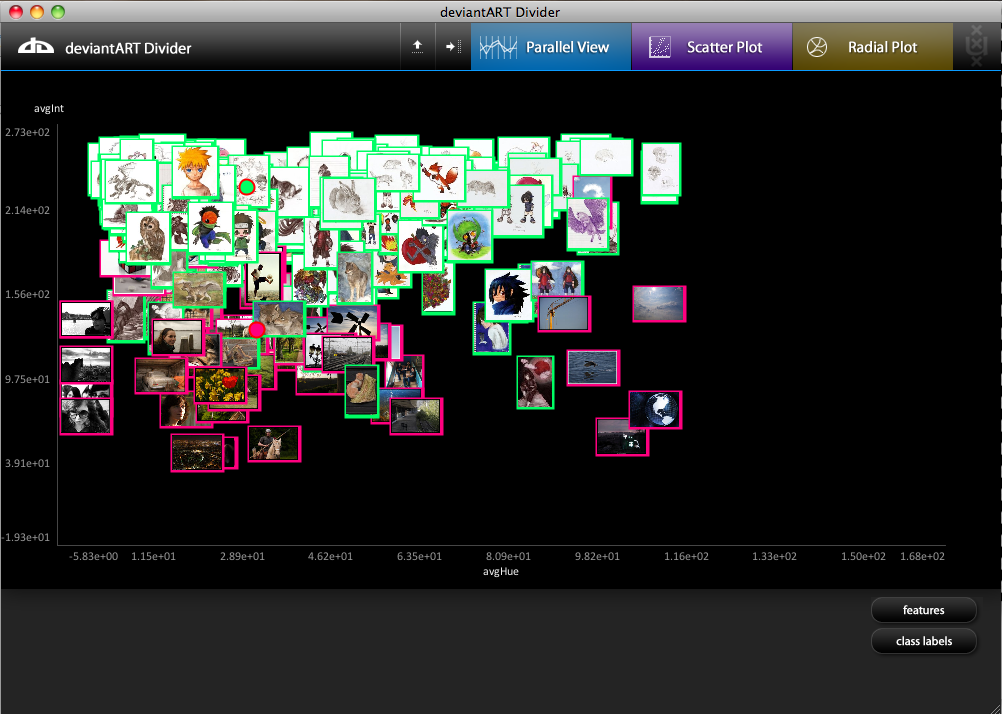
\includegraphics[width=1\linewidth]{img/visualization_scatter.png}
  \caption{The visualization application displaying a scatter plot of 2 artists.}
  \label{fig:visualization_scatter}
\end{figure}

Fig.~\ref{fig:visualization_scatter} shows the \textit{scatter plot} visualization technique.
The scatter plot displays values for two variables, which are image features that has been computed by the \textit{Feature extraction} component.
The data is displayed as a collection of miniature images.
Each having the value of one feature determining the position on the horizontal axis and the value of the other feature determining the position on the vertical axis.
The border around each image represents the class (artists or category) to which an image belongs.
For example, the images with a green border belong to the artist Kitsunebaka91 and the images with a red pink border belong to the artist Woekan.
The user has full control over which classes are displayed in the visualization.
The users can also control which two features are used as variables on the horizontal and vertical axis of the scatter plot.
A single image or all the images belonging to one class can be highlighted, making it more easy to recognize patterns.
The full version of a miniature image can be displayed to inspect it in more detail.

\begin{figure}[htb]
  \centering
  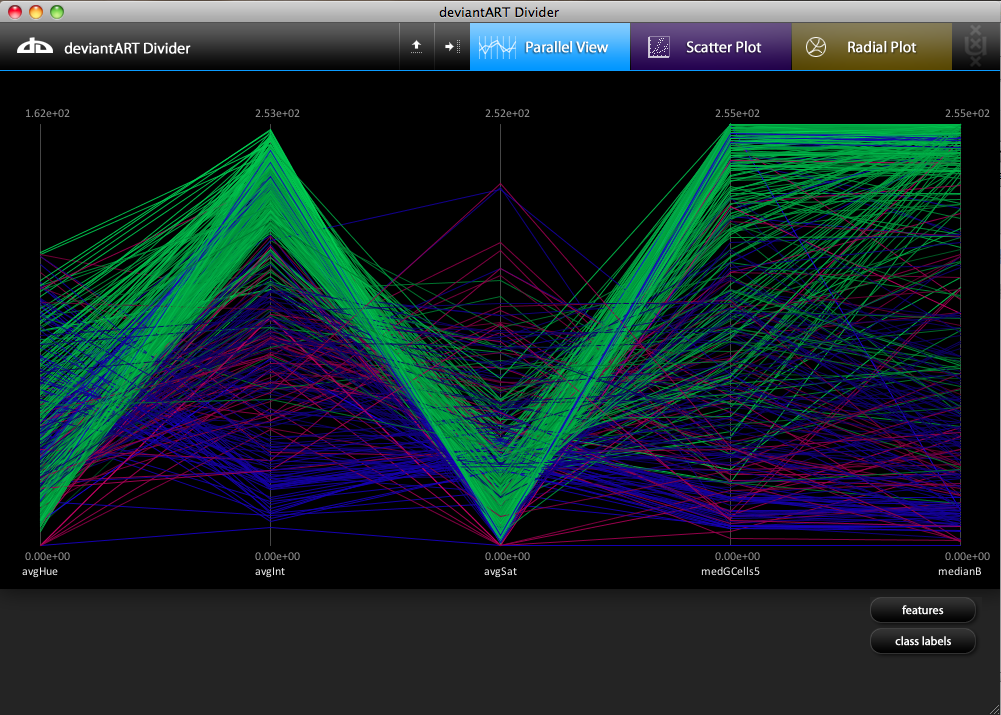
\includegraphics[width=1\linewidth]{img/visualization_parallel.png}
  \caption{The visualization application displaying a parallel coordinates plot of 3 artists and 5 features.}
  \label{fig:visualization_parallel}
\end{figure}

The scatter plot is limited to displaying only two features at the same time.
Fig.~\ref{fig:visualization_parallel} shows the \textit{parallel coordinates} visualization technique~\cite{andrienko2001constructing}, a common way of visualizing high-dimensional.
This enabled us to visualize beyond two features at the same time.
The two axes of the scatter plot are now replaced by $n$ vertical parallel lines to represent $n$ features ($n$-dimensional space).
An image is now represented as a polyline with vertices on the parallel axes.
The color of a polyline represents the class (artist, category) to which an image belongs.

\begin{figure}[htb]
  \centering
  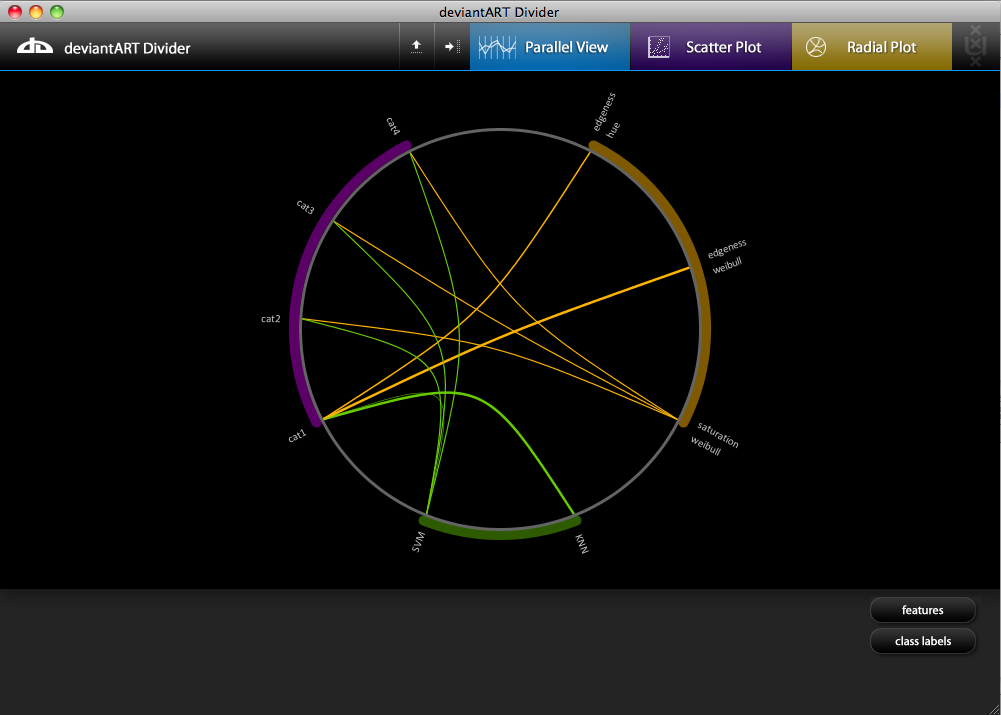
\includegraphics[width=1\linewidth]{img/visualization_radial.png}
  \caption{The visualization application displaying a radial plot that expresses the performance of the classification.}
  \label{fig:visualization_radial}
\end{figure}

Fig.~\ref{fig:visualization_radial} shows the \textit{radial plot} visualization technique.
This visualization is not used to visualize the dataset, but to display the performance of the classification, e.g., how a certain feature performs on separating an artist from the other artists.
The circle is split into three regions (variables): artists or categories (purple), features (yellow), classifiers (green).
%Each of these regions represent a variable that plays an important role in the classification of images.
%Each variables consists of a limited number of values that were used during classification.
The thickness of a line between two nodes expresses the performance of the classification when both nodes are used together, i.e., thicker lines means higher performance.
For example, a thick line between artist X and feature Y, means that feature Y is a good feature to separate artist X from the other artists.


\section{Experiments}
\subsection{Network experiments}
The network experiments have been performed to analyze the dA network and establish global characteristics of the network, but also to find interesting sub-networks of artists and artworks which are of particular interest to investigate.

The dA network consists of 13 million registered users, doing a full analysis of the the whole network was impossible within the scope of the project. Therefore a network of the dA watchers functionality\footnote{a watcher is someone who indicates he likes an artist and would like to receive updates when that artist produces new artwork.} was extracted for all but casual artists, these latter can be distinguished with a $~$, indicating that they do not have a paid membership. This network formed the basis of our network experiments.

From this large network of around 100'000 professional artists three core-networks were extracted using the findcore algorithm, described in Algorithm \ref{alg:findcore}. The three cores correspond to three types of the $degree(j)$ function in that algorithm, namely - in-degree, out-degree and in+out-degree -. This has resulted in a core of artists that are "power-watchers" a core with "popular-watched" artists and last a mix of both.

The results of the network experiments are presented in Table \ref{tab:netstatistics}, Table \ref{tabnetcooccurrences} as well as Figure \ref{fig:results_core}.  For all networks statistics were extracted, unfortunately for the large professional users network statistics such as the characteristic path length were not possible to compute within the given time period.

\begin{table}[htb]
    \centering
    \begin{tabular}
        { | l | c | c | c | c | c | c|} 
        \hline
        Network &  prof.  & watchers & watched & mixed\\
	            &  artists & core & core & core \\
        \hline
	no. nodes $(n)$& 103'663 & 1'701 & 1471 & 1099 \\
	no. links & 4'483'023 & 139'285 & 127'837  & 166'244 \\
	avg. degree $(k)$& 43.25 & 81.88 & 86.90 & 151.27 \\
	findcore $\max x$ & & 43 & 44 & 185\\
	$L_G$ & & 2.15 & 2.27 & 2.14 \\
	$L_{random}$ & & 1.69 & 1.63 & 1.40 \\
	$C_G$ & & 0.20 & 0.22 & 0.20 \\
	$C_{random}$ & & 0.048 & 0.059 & 0.140 \\
	\hline
    \end{tabular}
    \caption{Network statistics}
    \label{tab:netstatistics}
\end{table}
\begin{table}[htb]
    \centering
    \begin{tabular}
        { | l | c | c | c |} 
        \hline
        core Network & watchers & watched & mixed\\
        co-occurrences  &   core & core & core \\
        \hline
        watchers core & 1701 &541& 54\\
        watched core & 541 &1471& 286\\
        mixed core  &54 &286 &1099\\
	\hline
    \end{tabular}
    \caption{Core network co-occurrences, there are 14 artists which are in all 3 core networks}
    \label{tab:netcooccurrences}
\end{table}

\begin{figure*}[htb]
  \centering
  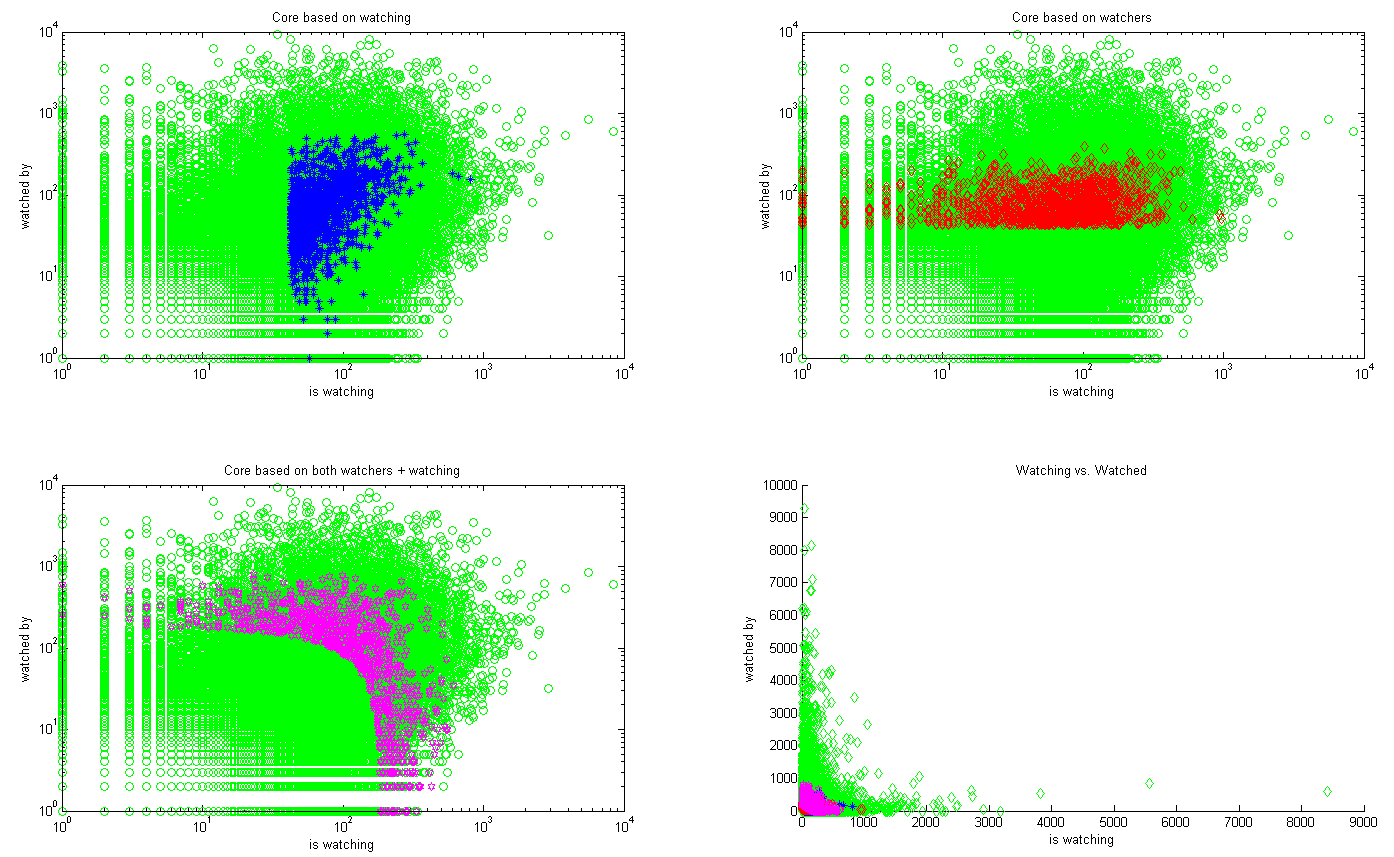
\includegraphics[width=1\linewidth]{img/core.png}
  \caption{Core networks, the degree of watching versus being watched.  The green dots represent the whole professional network, while the blue represents the watchers-core, red the watched and pink the mixed core, the last sub figure shows the power-law behavior of the degree distributions.}
  \label{fig:results_core}
\end{figure*}

Through application of the findcore algorithm we have been able to find cores of interesting users, which are of manageable size for full analysis. To establish if these core networks are small-world, we refer to the definition of small-world networks as described in section \ref{net_proposed_approach}, a network can be considered small-world when $L_G\approx L_{random}$ and $C_G \gg C_{random}$. All core networks have a clustering coefficient larger than a comparable random network, though the mixed core is close to the random network. The characteristic path lengths are longer than their random network equivalents. This is most likely due to the relatively small size of the networks, the paths are still significantly smaller than $L_{lattice}=\frac{n}{2k}$. We therefore conclude that the core's of dA can be considered small-world networks.  
Furthermore the co-occurrences between the watchers and watched network is about $\frac{1}{3}$, while this is much lower for the mixed network. We presume that this has to do with the findcore degree $\max x$ which is much higher for the mixed network. Thus the mixed network is distinct from the watchers and watched cores which are more alike.



\subsection{Image experiments}
For the image experiments we collected our dataset by downloading the complete galleries from around 30 artists.
Those artists were selected from the daily deviations of a random day and includes both premium and non premium members.
In total we downloaded around 5000 images. 
For each image we also stored the category information.
The dataset is unbalanced since some artists only have around 50 images, while other artists have over 500 images.
Some more detailed statistics about the dataset are listed in table \ref{datasetstats}.


\begin{table}[htb]
    \caption{Dataset artist statistics}
    \label{datasetstats2}
\end{table}

\begin{figure}[htb]
%  \centering
  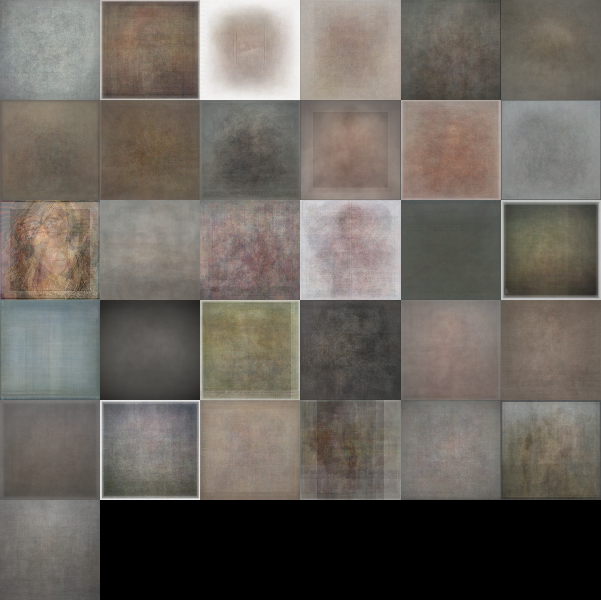
\includegraphics[width=1\linewidth]{img/datasetAvg.png}
  \caption{mean image per artist, left to right, top to bottom, in order of table \ref{datasetstats2}: Craniata, K1lgore, Kitsunebaka91, ..., zihnisinir }
  \label{fig:avgDataset}
\end{figure}


\begin{table}[ht]
	\centering

	\subtable[General statistics]{
		\begin{tabular} { |l|c| }
			\hline
			Total Size & 1.4gb \\
			\hline
			Users & 31 \\
			\hline
			Image count & 5324 \\
			\hline 
			Average image width & 671 \\
			\hline
			Average image height & 689 \\
			\hline
			Average image size & 250kb \\
			\hline
			Average image count & 171 \\
			\hline
		\end{tabular}
	}

	\subtable[Artist image statistics]{
		\begin{tabular}
		    { | l | c | l | c|} 
		    \hline
		    Name & count & Name & count \\
		    \hline
		Craniata &  61 & K1lgore & 63 \\
		Kitsunebaka91 & 272  & Knuxtiger4 & 193 \\
		LALAax & 82  & Mallimaakari & 151 \\
		Mentosik8 & 110 & NEDxfullMOon & 116 \\
		One-Vox & 74 & Pierrebfoto & 188 \\
		Red-Priest-Usada & 132 & Skarbog & 229 \\
		Swezzels & 9 & Udodelig & 54 \\
		UdonNodu & 38 & WarrenLouw & 51 \\
		catluvr2 & 793 & erroid & 146 \\
		fediaFedia & 303 & gsphoto & 661 \\
		iakobos & 47 & kamilsmala & 39 \\
		miss-mosh & 307 & nyctopterus & 68 \\
		omega300m & 483 & sekcyjny & 55 \\
		stereoflow & 166 & sujawoto & 33 \\
		wirestyle & 143 & woekan & 49 \\
		zihnisinir & 177 \\

		    \hline 
		\end{tabular}
	}

	\subtable[Category statistics]{
		\begin{tabular}
		    { | l | c | } 
		    \hline
		    Category & count \\
		    \hline
		    photography & 2244 \\ 
		    customization & 906 \\ 
		    traditional & 842 \\ 
		    digitalart & 587 \\ 
		    fanart & 239 \\ 
		    \hline 
		\end{tabular}
		}
    \caption{Dataset statistics}
    \label{datasetstats}
\end{table}

%\subsubsection{Experiment 1: One against all artists}

%The first experiment using this toolkit is to find out if there are any artists in our dataset that uses an unique style.
%The experiment is performed using two feature combination, the statistical features and the cognitive features.
%Also it is focused on using one artist as the positive class while all the other artists are in the negative class resulting in a two class problem.
%This experiment is set up as an orientation experiment to find out what might work for this dataset and what might not.
%Also this experiment can give a clear indication of how to approach this type of dataset.
%
%For this experiment, three classifiers were used: kNN, Naive Bayes and the Nearest Mean classifiers.
%The classifiers were trained on a train set which consists of 70\% of the entire dataset.
%Training was done with a 5 fold cross-validation and the performance of each classifier can be computed by calculating the average of the $F_1$-measure gathered from all folds.
%Because this is an orientation experiment, no test set was incorporated in this experiment.
%
%%\subsubsection{Experiment 1: Results}
%
%%\begin{table*}
%%    \centering
%%    \begin{tabular}
%%        { | l | l | c | c |} 
%%        \hline
%%        Artist & Classifier & Parameter & F-Measure \\
%%        \hline
%%        my\_shots & Nearest Mean & - & 0.8742 \\ 
%%        gsphoto & kNN & 3 & 0.8722 \\ 
%%        gsphoto & kNN & 5 & 0.8711 \\ 
%%        Pierrebfoto & Naive Bayes & 10 & 0.8698 \\ 
%%        Kitsunebaka91 & Naive Bayes & 24 & 0.8693 \\
%%        Kitsunebaka91 & Naive Bayes & 12 & 0.8680 \\
%%        gsphoto & kNN & 7 & 0.8669 \\
%%        Kitsunebaka91 & Naive Bayes & 22 & 0.8668 \\
%%        gsphoto & kNN & 9 & 0.8664 \\
%%        Kitsunebaka91 & Naive Bayes & 8 & 0.8657 \\
%%        \hline 
%%    \end{tabular}
%%    \caption{Top 10 Ranking of the highest $F_1$-measure using \textit{statistical features}}
%%    \label{ex1aresults}
%%\end{table*}
%
%\begin{table}[htb]
%    \centering
%    \begin{tabular}
%        { | l | l | c |} 
%        \hline
%        Artist & Classifier & $F_1$-Measure \\
%        \hline
%        my\_shots & Nearest Mean & 0.8742 \\ 
%        gsphoto & kNN & 0.8722 \\ 
%        gsphoto & kNN & 0.8711 \\ 
%        Pierrebfoto & Naive Bayes & 0.8698 \\ 
%        Kitsunebaka91 & Naive Bayes & 0.8693 \\
%        Kitsunebaka91 & Naive Bayes & 0.8680 \\
%        gsphoto & kNN & 0.8669 \\
%        Kitsunebaka91 & Naive Bayes & 0.8668 \\
%        gsphoto & kNN & 0.8664 \\
%        Kitsunebaka91 & Naive Bayes & 0.8657 \\
%        \hline 
%    \end{tabular}
%    \caption{Top 10 Ranking of the highest $F_1$-measure using \textit{statistical features}}
%    \label{ex1aresults}
%\end{table}
%
%The results from the experiment for the statistical features can be found in table \ref{ex1aresults}.
%The table lists the top 10 ranking of the artist names combined with the classifier and parameter used to train the classifier.
%The ranking is in a descending order starting from the combination that performed the best according to the $F_1$-measure.
%
%The table shows that 2 artist names exists multiple times in the top 10 ranking.
%Those artists are \textit{Kitsunebaka91} and \textit{gsphoto} and the table shows that they were separated from all other artists using different classifiers and parameter settings.
%
%The table also shows that the nearest mean classifier only has one entry in the top 10.
%Eventhough it has the highest $F_1$-measure, the classifier does not seem to be performing well on the other artists.
%
%%\begin{table*}
%%    \centering
%%    \begin{tabular}
%%        { | l | l | c | c |} 
%%        \hline
%%        Artist & Classifier & Parameter & F-Measure \\
%%        \hline
%%        giannisgx89 & Nearest Mean & - & 0.8549 \\ 
%%        gsphoto & Nearest Mean & - & 0.8196 \\ 
%%        Pierrebfoto & Nearest Mean & - & 0.7305 \\ 
%%        sekcyjny & Nearest Mean & - & 0.7298 \\ 
%%        fediaFedia & Nearest Mean & - & 0.7133 \\
%%        NEDxfullMOom & Nearest Mean & - & 0.7020 \\
%%        erroid & Nearest Mean & - & 0.6831 \\
%%        gsphoto & Naive Bayes & 14 & 0.6820 \\
%%        Mentosik8 & Nearest Mean & - & 0.6801 \\
%%        gsphoto & Naive Bayes & 10 & 0.6753 \\
%%        \hline 
%%    \end{tabular}
%%    \caption{Top 10 Ranking of the highest $F_1$-measure using \textit{cognitive} features}
%%    \label{ex1bresults}
%%\end{table*}
%
%\begin{table}[htb]
%    \centering
%    \begin{tabular}
%        { | l | l | c |} 
%        \hline
%        Artist & Classifier & $F_1$-Measure \\
%        \hline
%        giannisgx89 & Nearest Mean & 0.8549 \\ 
%        gsphoto & Nearest Mean & 0.8196 \\ 
%        Pierrebfoto & Nearest Mean & 0.7305 \\ 
%        sekcyjny & Nearest Mean & 0.7298 \\ 
%        fediaFedia & Nearest Mean & 0.7133 \\
%        NEDxfullMOom & Nearest Mean & 0.7020 \\
%        erroid & Nearest Mean & 0.6831 \\
%        gsphoto & Naive Bayes & 0.6820 \\
%        Mentosik8 & Nearest Mean & 0.6801 \\
%        gsphoto & Naive Bayes & 0.6753 \\
%        \hline 
%    \end{tabular}
%    \caption{Top 10 Ranking of the highest $F_1$-measure using \textit{cognitive} features}
%    \label{ex1bresults}
%\end{table}
%
%Table \ref{ex1bresults} shows the results obtained from only using cognitive features to separate artists from each other.
%In contrast to table \ref{ex1aresults} these results show that the nearest mean classifier is the one having the best performance according to $F_1$-measure.
%
%However using cognitive features results into a different ranking of separable artists, the performance of each classifier is not as high as for using statistical features.
%The top 10 ranking using the statistical features all have scores above the 0.8 indicating that using statistical features seems more stable compared to using cognitive features.
%
%This orientation experiment showed that using statistical features better results can be obtained compared to using cognitive features.
%Also it seems like there are some artists that can be seperable from all the others but most artists do not perform well in this experiment.
%Using the results of this experiment it is hard to describe why this is happening. 
%An experiment showing which features contributes to the separation of an artist from all other artists is important in order to describe why the style of an artist is unique compared to the other artists in the dataset.
%The next section describes an experiment that gives a clear view over these questions.

\subsubsection{Experimental Setup}

This experiment is focused on finding the most defining features of every artist in the dataset.
For every artist, the feature selection algorithm selects the best 5 features that according to the inter-intra criterion can separate that artist with another artist.
This will be done for every artist pair that can be found in the dataset, meaning that the best 5 features can differ depending on what kind of artist pair is used.

At first, a classifier needs to be selected which is going to be used to give a performance score for each set of features that the feature selection algorithm is computing.
The classifier is selected by optimizing the parameters for each classifier using 5 fold cross-validation on the training set, which is 70 percent of the dataset.
The classifier selected will be the one that gives the highest performance score.

For every artist pair a performance score is computed based on how well the selected classifier can separate those artists given the features.
Therefore the performance measure used here is the $F_1$-measure.

%For this experiment each artist is compared to one other artist.
%The motivation of this approach is that each artist can be evaluated separately and it can give more clarity for cases where the performance of a classifier is low.
%The experiment is done for all the artists in the dataset meaning that an artist is compared to every other artist in the dataset.
%Also this experiment uses the feature selection algorithm to determine the features that best separates an artist from another artist.
%The feature selection algorithm selects features up to a combination of 5 different features for every artist pair.
%
%For this experiment the kNN, Naive Bayes, Nearest Mean and the SVM classifiers were optimized and trained on the train set using 5 fold cross-validation and the highest average $F_1$-measure determines the classifier that is used to produce the results.
%
%For every artist pair the $F_1$-measure is calculated on the test set to evaluate the performance of the classifier separating those artists.

\subsubsection{Image Experiment Results}

\begin{table}[htb]
    \centering
    \begin{tabular}
        { | l | c | c |} 
        \hline
        Classifier & Mean $F_1$-measure & Stddev $F_1$-measure  \\
        \hline
        kNN & 0.7074 & 0.1731 \\ 
        Naive Bayes & 0.7897 & 0.1030 \\ 
        Nearest Mean & 0.7383 & 0.1086 \\ 
        Linear SVM & 0.8278 & 0.1450 \\ 
        \hline 
    \end{tabular}
    \caption{The mean $F_1$-measure and the standard deviation performance score of each optimized classifier on the train set using 5-fold cross-validation}
    \label{ex2optimizeresults}
\end{table}

The results of optimizing the classifiers and then validating them using the train set are shown in table \ref{ex2optimizeresults}.
The results show that the linear SVM has got the highest mean $F_1$-measure score and also the second highest standard deviation.
Based on these scores, it is best to select the linear SVM to assign performance scores because this classifier can best separate artists.

%Table \ref{ex2optimizeresults} shows the results After the optimization and training of the classifiers.
%The linear SVM classifier obtained the highest average $F_1$-measure however the Naive Bayes classifier did not perform significantly worse than the SVM.
%Note that the main goal of this experiment is to find feature combinations that distinguish artists.
%Therefore the focus should not go to maximizing the $F_1$-measure on the test set meaning that one classifier should be enough for this type of task.

\begin{figure*}[htb]
  \centering
  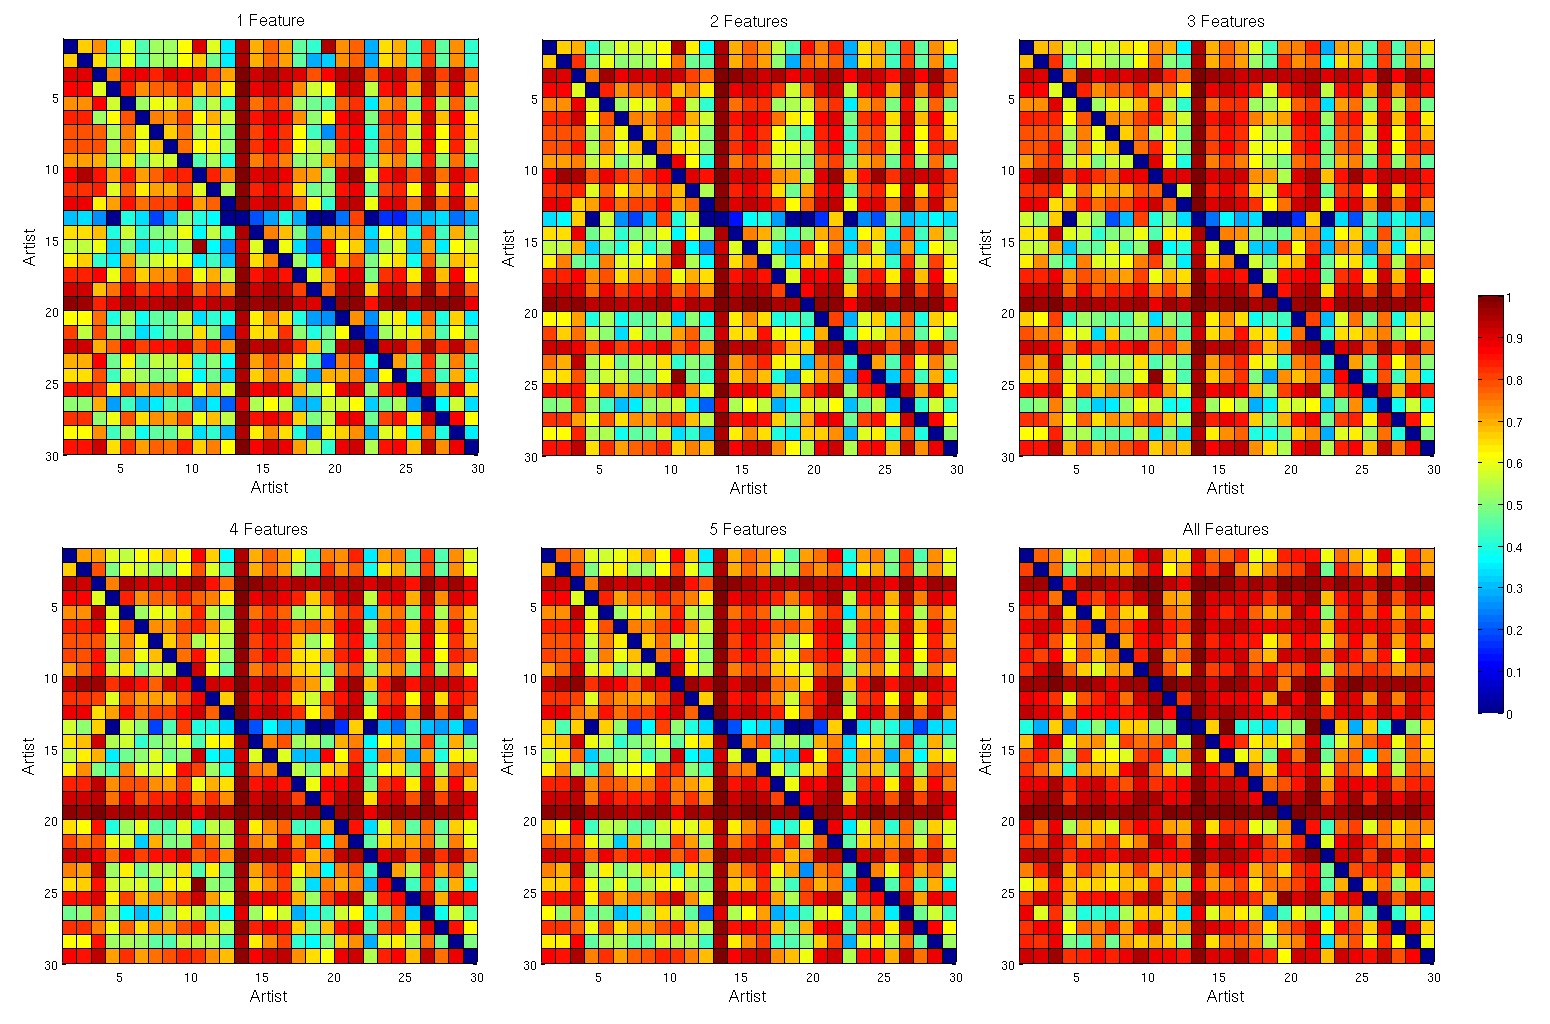
\includegraphics[width=0.75\linewidth]{img/experiment2results.png}
  \caption{The intensity mapping of the results using the linear SVM in combination with different sets of features.
  The mapping is divided into 30x30 squares where each square represents the $F_1$-measure of artist x with artist y.
  The artists are represented on both the x and the y axis by numbers.
  Table \ref{ex2stats} shows which artists are corresponding to which number.
  Also the red color represents the highest value($F_1$-measure=1).
  In the upperleft mapping, the performance using only \textit{the most} informative feature according to the selection algorithm is mapped.
  In the upperright mapping, the performance of using the \textit{3} most informative features are mapped.
  In the lowerleft mapping, the performance of using the \textit{5} most informative features are mapped.
  In the lowerright mapping, the performance of using \textit{all} the features are mapped.
  }
  \label{fig:experiment2results}
\end{figure*}

The results of using the trained linear SVM on the test set is shown in figure \ref{fig:experiment2results}.
The figure shows the intensity mappings of different lengths of feature sets.
It shows that the length of the feature sets used to separate artists is correlated to the performance score between them.
It also shows that there are artists pairs that can be separated using only a few features.
There are even artists which can be separated from every other artist in the dataset.
This is shown by the columns and rows that are predominantly red.
These artists uses an art style that is unique compared to the other artists in this dataset.
This result tells that those artists can be described using the features that were created using this toolkit.

\begin{table*}[htb]
    \centering
    \begin{tabular}
        { | c | l | c | c | l | } 
        \hline
        No. & Name & mean $F_1$-measure & stddev $F_1$-measure & Most defining features\\
        \hline
    1 & Craniata &  0.6314 & 0.1864 & Center average Hue, Center corner detection, Center edge detection\\
    2 & K1lgore & 0.6078 & 0.1813 & Entropy of the Intensity, Variance of the Intensity, Edge detection \\
    3 & Kitsunebaka91 & 0.8827 & 0.1756 & Center edge detection, Entropy of the Intensity, Edge detection \\
    4 & Knuxtiger4 & 0.7751 & 0.1822 & Variance of the Intensity, Entropy of the Intensity, Center edge detection \\
    5 & LALAax & 0.6498 & 0.1902 & Edgeratio, Entropy of the Intensity, Variance of the Intensity \\
    6 & Mallimaakari & 0.7548 & 0.1824 & Variance of the Intensity, Center edge detection, Center average Hue\\
    7 & Mentosik8 & 0.6807 & 0.1876 & Entropy of the Intensity, Variance of the Intensity, Lowerleft edge detection \\ 
    8 & NEDxfullMOon & 0.7071 & 0.1880 & Center edge detection, Center avg B, Entropy of the Intensity\\
    9 & One-Vox & 0.6570 & 0.1833 & Entropy of the Intensity, Edge detection, Center edge detection  \\
    10 & Pierrebfoto & 0.8375 & 0.1852 & salMapKEntropy, Center average Hue, Edge detection\\
    11 & Red-Priest-Usada & 0.7376 & 0.1851 & salMapIEntropy, Center Edge detection, salMapOEntropy\\
    12 & Skarbog & 0.7875 & 0.1869 & Entropy of the Intensity, Center average saturation, Lowerright average R \\
    13 & Swezzels & 0.3296 & 0.2281 & - \\ 
    14 & Udodelig & 0.5798 & 0.1887 & Entropy of the Saliency, Entropy of the Intensity, salhistdev \\
    15 & UdonNodu & 0.5352 & 0.2158 & SalmapOentropy, Variance of the Intensity, Uppermiddel average Hue \\ 
    16 & WarrenLouw & 0.6235 & 0.1864 & Entropy of the Intensity, median B, Upperright median Intensity\\
    17 & erroid & 0.7535 & 0.1833 & Variance of the Intensity, Center edge detection, Entropy of the Intensity\\
    18 & fediaFedia & 0.8270 & 0.1804 & Center edge detection, corner detection, Variance of the Intensity \\
    19 & gsphoto & 0.9172 & 0.1779 & Entropy of the Intensity, Variance of the Intensity, Center edge detection \\
    20 & iakobos & 0.5764 & 0.1899 & Edge detection, upperleft average saturation, upperleft median G \\
    21 & kamilsmala & 0.6359 & 0.1978 & Variance of the Intensity, Entropy of the Intensity, middleleft edge detection\\
    22 & miss-mosh & 0.8205 & 0.1811 & upperleft corner detection, Number of faces, Entropy of the Intensity \\
    23 & nyctopterus & 0.6324 & 0.1950 & Variance of the Intensity, Center median Hue, center average Hue\\
    24 & sekcyjny & 0.5875 & 0.1983 & Entropy of the Intensity, Downmiddle edge detection, salmapOEntropy\\
    25 & stereoflow & 0.7576 & 0.1904 & Center average Hue, Variance of the Intensity, Corner detection \\
    26 & sujawoto & 0.4752 & 0.1873 & SalmapIEntropy, Entropy of the Intensity, Downmiddle edge detection\\
    27 & wirestyle & 0.7138 & 0.1931 & SalmapIEntropy, Variance of the Intensity, Center average B\\ 
    28 & woekan & 0.5529 & 0.1881 & Entropy of the Intensity, Variance of the Intensity, Upperleft edge detection\\
    29 & zihnisinir & 0.7632 & 0.1918 & Entropy of the Intensity, Center average saturation, SalMapIEntropy\\
    30 & omega300m & 0.8318 & 0.2403 & Entropy of the Intensity, Center edge detection, Downright average Intensity \\
        \hline 
    \end{tabular}
    \caption{This table first describes the mean $F_1$-measure and its standard deviation for every artist which was computed by using linear SVM combined with a feature set containing the 5 most informative features that separates an artist pair.
    It also shows the number of the artist that corresponds to the x/y axis of the intensity mappings found in figure \ref{fig:experiment2results}.
    The last column shows the most defining features that can describe the artist.}
    \label{ex2stats}
\end{table*}

Table \ref{ex2stats} shows the summary of this experiment and it shows what the most defining features are for each artist.
Note that some artists, according to the feature selection algorithm, contains defining features but the mean $F_1$-measure is very low.
This shows that eventhough they are the defining features, one should not assume that they can describe the artist.
The classifier could not correctly separate the artist from the other artists by using those features.
The mean $F_1$-measure can be seen as the score that these features are in fact correctly describing the artist.

The table also shows that the edge detection and the intensity are valuable features in describing artist styles.
This is very feasible because images can actually range between being dark and very light and also there are styles where there are a lot of edges like in photographs or drawings but other styles like abstract can have very little edges.
Other features that can be found in this table are the hue and corner detection but they are not used as much as the edge detection and the intensity.

Also it seems that cognitive features work best in certain types of styles.
In this dataset, the artist $Pierrebfoto$ has a lot of nude images and this was picked up using the skin map feature.

Another important detail about these results is that the center cell of an image is chosen a lot compared to the other cells.
This is actually highly feasible because most of the time in an image, the center contains the most information.

These results have shown that some artists can be described by only a using a few features.
Also edge detection and intensity are important features that can be considered when describing artists. 

%Figure \ref{fig:experiment2results} shows the results for this experiment using the linear SVM which was chosen in a greedy fashion based on the results found in table \ref{ex2optimizeresults}.
%From left to right the figure shows the results of using: \textit{1} feature, \textit{2} features, \textit{3} features, \textit{4} features, \textit{5} features and \textit{all} features as the feature combination that is used by the classifier to classify images.
%The results are plotted using an intensity mapping where each square represents the $F_1$-measure performance of separating the \textit{x} and \textit{y} artist.
%
%The first thing that is noticable is that the intensity mappings are not symmetric.
%This is because the $F_1$-measure was used here to evaluate the performance.
%The measure is calculated by looking at the precision and recall of the positive class, so when the classes are turned around the $F_1$-measure will also turn into a different value.
%Therefore in order to determine if two artists are separable, there is a need to look at the $F_1$-measure for both artists.
%This is because for some artist pairs the $F_1$-measure of one artist has a value of 1 while the other has a value of 0.
%This means that for those artist pairs the classifier has classified all images to one artist, which most of the time is caused by the non-uniform dataset.
%
%Furthermore the figure shows that artists can be better separated by using more features.
%The intensity mapping using all features shows that it has the highest overall $F_1$-measure.
%However the more interesting mappings are the ones where only the top 1,2,3,4,5 features were used for classification.
%Eventhough their performance is lower than using all the features it gives information about the most defining features that is used to separate an artist from another artist.
%
%The intensity mappings using 1 to 5 features contains artists that have an overall high $F_1$-measure which shows that some artists can be separated from all other artists using only a few features.
%
%\begin{table}[htb]
%    \centering
%    \begin{tabular}
%        { | l | c |} 
%        \hline
%        Feature & Counts \\
%        \hline
%        gridEdgeRatio\_5 & 9 \\ 
%        intEntropy & 4 \\ 
%        edgeRatio & 4 \\ 
%        avgRCells\_9 & 4 \\ 
%        medIntCells\_2 & 3 \\
%        medIntCells\_7 & 3 \\
%        \hline 
%    \end{tabular}
%    \caption{Counts of features that were used to separate \textit{Kitsunebaka91} from the other artists.}
%    \label{kitsune}
%\end{table}
%
%Table \ref{kitsune} shows the top 6 feature counts of features that were used to distinct \textit{Kitsunebaka91} from the other artists.
%The features were counted whenever the $F_1$-measure of \textit{Kitsunebaka91} had an $F_1$-measure higher than 0.9, which indicates that the artist is separable from the other artist.
%So the table details the reason why \textit{Kitsunebaka91} was separable.
%The artwork of \textit{Kitsunebaka91} consists mostly of images where there is a white background with a drawing in the center of it.
%This corresponds to the features found using this toolkit because table \ref{kitsune} shows that the edgeratio and intensity of the images are the dominant features to separate this artist from other artists.
%Also the table shows that the \textit{GridEdgeRatio\_5} feature is used multiple times to separate this artist.
%This again corresponds to the artist style because the \textit{GridEdgeRatio\_5} is the edgeratio value of the center cell of an image, the cell where the drawing of the artist lies.
%
%Eventhough \textit{Kitsunebaka91} was seperable from most other artists, pairing \textit{Kitsunebaka91} with the artist \textit{Knuxtiger4} resulted in a lower $F_1$-measure of 0.7397 wheras the mean of all the scores was 0.91.
%Inspecting the images of \textit{Knuxtiger4} showed that the artist mostly contained images that were drawings on a white background similar to that of \textit{Kitsunebaka91}.
%Therefore it is not surprising that the score for that pair was lower than the average because the classifier could not seperate those images.
%These results indicates that these results can be used to create a recommender system.



\section{Future work}
%Use network better to guide our research, use network to pick dataset.
%recommender system
%doing it on a different dataset

%\begin{itemize}
\subsubsection{more features - this header can later be removed}
%\item More features, Including emotional features (color and texture)
It could be interesting to increase the number of extracted features, especially the ones coming from anlysis of human perceptions.
For instance, the emotional impact of an artwork plays a significant role in the artistic creative process, and therefore the extraction of emotion-inspired features, such as color weight, color activity and color heat \cite{color_emotion1} could help the classifier to better distinquish betweent classes. Moreover, the inclusion of texture would give an even deeper emotional descriptor \cite{LucassenECCGIV2010}. 
%\item More network information - Using the Core network as a basis for a new dataset (ongoing), More links, not only watchers (hierachy)
\subsubsection{more network- this header can later be removed}
We want to expand the network to include more than only "watcher-watching" connections. DeviantArt is a rich dataset from which we can also extract the "artist-artwork", "artwork-hierarchical class", "hierarchiecal taxonomy" -connections, as well as comments users make to artists and/or pictures. 
Since our current investigations have provided us with a managable set of core users for deviantArt, this group can guide us in dataset collection for future work. Relevant questions can be, how the hierarchical artwork classification relates to sub-networks in the core of artists producing artwork in a particular class. Another relevant question is if the network structure and artwork in the core is representative for the whole network. If we can identify different usage patterns of DeviantART, for instance 'hubs' which are artists who are not popular because of the artwork thei themselve produce. But because of the other artists they connect to versus original artists who are popular because of their own work.

 
%\item Incorporating time
%\item Using classifiers to make recommendations
%\end{itemize}

\section{Conclusion}
conclusion

%\appendix
%\section{Datasets}
%%\subsection{Image Dataset}

\begin{table}[htb]
    \centering
    \begin{tabular}
        { | l | c | l | c|} 
        \hline
        Name & count & Name & count \\
        \hline
    Craniata &  61 & K1lgore & 63 \\
    Kitsunebaka91 & 272  & Knuxtiger4 & 193 \\
    LALAax & 82  & Mallimaakari & 151 \\
    Mentosik8 & 110 & NEDxfullMOon & 116 \\
    One-Vox & 74 & Pierrebfoto & 188 \\
    Red-Priest-Usada & 132 & Skarbog & 229 \\
    Swezzels & 9 & Udodelig & 54 \\
    UdonNodu & 38 & WarrenLouw & 51 \\
    catluvr2 & 793 & erroid & 146 \\
    fediaFedia & 303 & gsphoto & 661 \\
    iakobos & 47 & kamilsmala & 39 \\
    miss-mosh & 307 & nyctopterus & 68 \\
    omega300m & 483 & sekcyjny & 55 \\
    stereoflow & 166 & sujawoto & 33 \\
    wirestyle & 143 & woekan & 49 \\
    zihnisinir & 177 \\

        \hline 
    \end{tabular}
    \caption{Dataset artist statistics}
    \label{datasetstats2}
\end{table}

\begin{figure*}[htb]
  \centering
  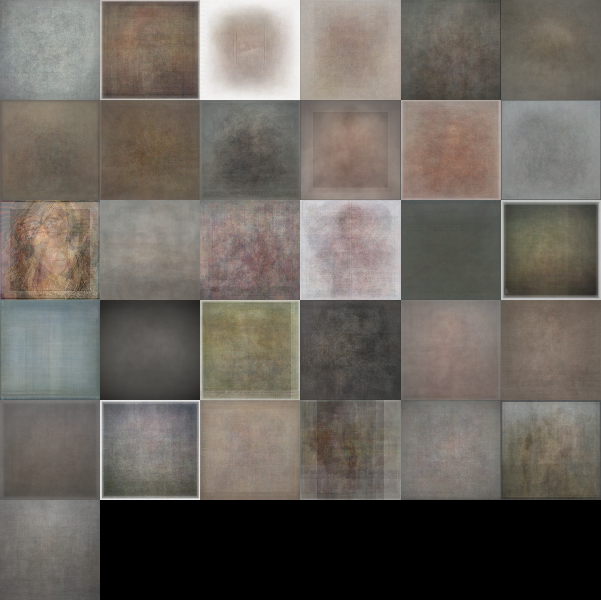
\includegraphics[width=1\linewidth]{img/datasetAvg.png}
  \caption{mean image per artist, left to right, top to bottom: Craniata, K1lgore, Kitsunebaka91, ..., zihnisinir }
  \label{fig:avgDataset}
\end{figure*}

%\nocite{*}
\bibliographystyle{unsrt}
\bibliography{bibtex}

\pagebreak
\tableofcontents

\end{document}